\chapter{Instantiating a cognitive model for predicting vehicle behavior}
\label{chap:behav_pred}

Predicting future behavior and positions of other traffic participants from observations is a key problem, that needs to be solved by human drivers and automated vehicles alike to safely navigate their environment and to reach their desired goal.
Therefore, we picked behavior prediction as another task for investigating the potential of vector representations in automotive context.
In contrast to the previous task of classifying the current driving context (cf. Sec.~\ref{sec:driving_context_class}), predicting future positions of vehicles is a regression problem, as we are predicting continuous values (spatial positions) instead of discrete labels.
However, future positions of vehicles not only depend on each vehicle's own past positions and dynamic data (e.g. velocity and acceleration) but also on the behavior of the other traffic participants in the vehicle's surroundings.
We hypothesize that structured vector representations will be able to capture these relations and mutual influence between traffic participants, which is necessary for reliable predictions.
As we aim for a model-free data representation, we avoid introducing any physical constraints or restrictions regarding our data-representation or the predicting models.
Although this allows for physically unrealistic or even impossible trajectory predictions, we want our neural network models to figure out the best predictions on their own without biasing them in any direction.
In this section, we present a representation of spatial information for multiple objects in semantic vectors of fixed length using the convolutive power introduced in def.~\ref{def:conv_power}. 
We use this representation as input for simple feedforward neural networks and more sophisticated \ac{LSTM}-based models and compare them against each other and a linear predictor as the simplest baseline.
We conduct a thorough and detailed analysis for all of these models and show that by using our vector representation with a simple network architecture we can achieve results comparable to more complex models.

\section{Data and preprocessing}
\label{sec:data_preproc}

% \begin{figure}[t!]
% 	\centering
% 	\includegraphics[width=\textwidth]{imgs/figure4.jpg}
% 	\caption{Data visualization of one driving situation example from the \emph{On-board} data-set $D_1$ \textbf{(A)} and one example from the \emph{\acs{NGSIM}} data-set $D_2$ \textbf{(B)}. The dots indicate the position of the vehicles and color-code the vehicle type (red=motorcycle, green=car, blue=truck, black=ego-vehicle), blue and orange lines show past and future motion of the target vehicle whereas gray lines depict the other vehicles' motion.}\label{fig:data_example}
% \end{figure}
In this thesis, we use two different data-sets for training and evaluation of our behavior preidction models, which we describe in more detail in the subsequent sections.
We refer to those data-sets as \emph{On-board} or $D_1$ (see Sec.~\ref{subsec:onboard-dataset}), which is our main data-set, and \emph{\acs{NGSIM}} or $D_2$ (see Sec.~\ref{subsec:ngsim-dataset}), which is a publicly available data-set used for reference and comparability.
In this section, we describe both data-sets regarding available features, available sources of information as well as their key differences and the preprocessing procedure.

\subsection{On-board-sensors data-set}
\label{subsec:onboard-dataset}

\begin{figure}[t!]
	\centering
	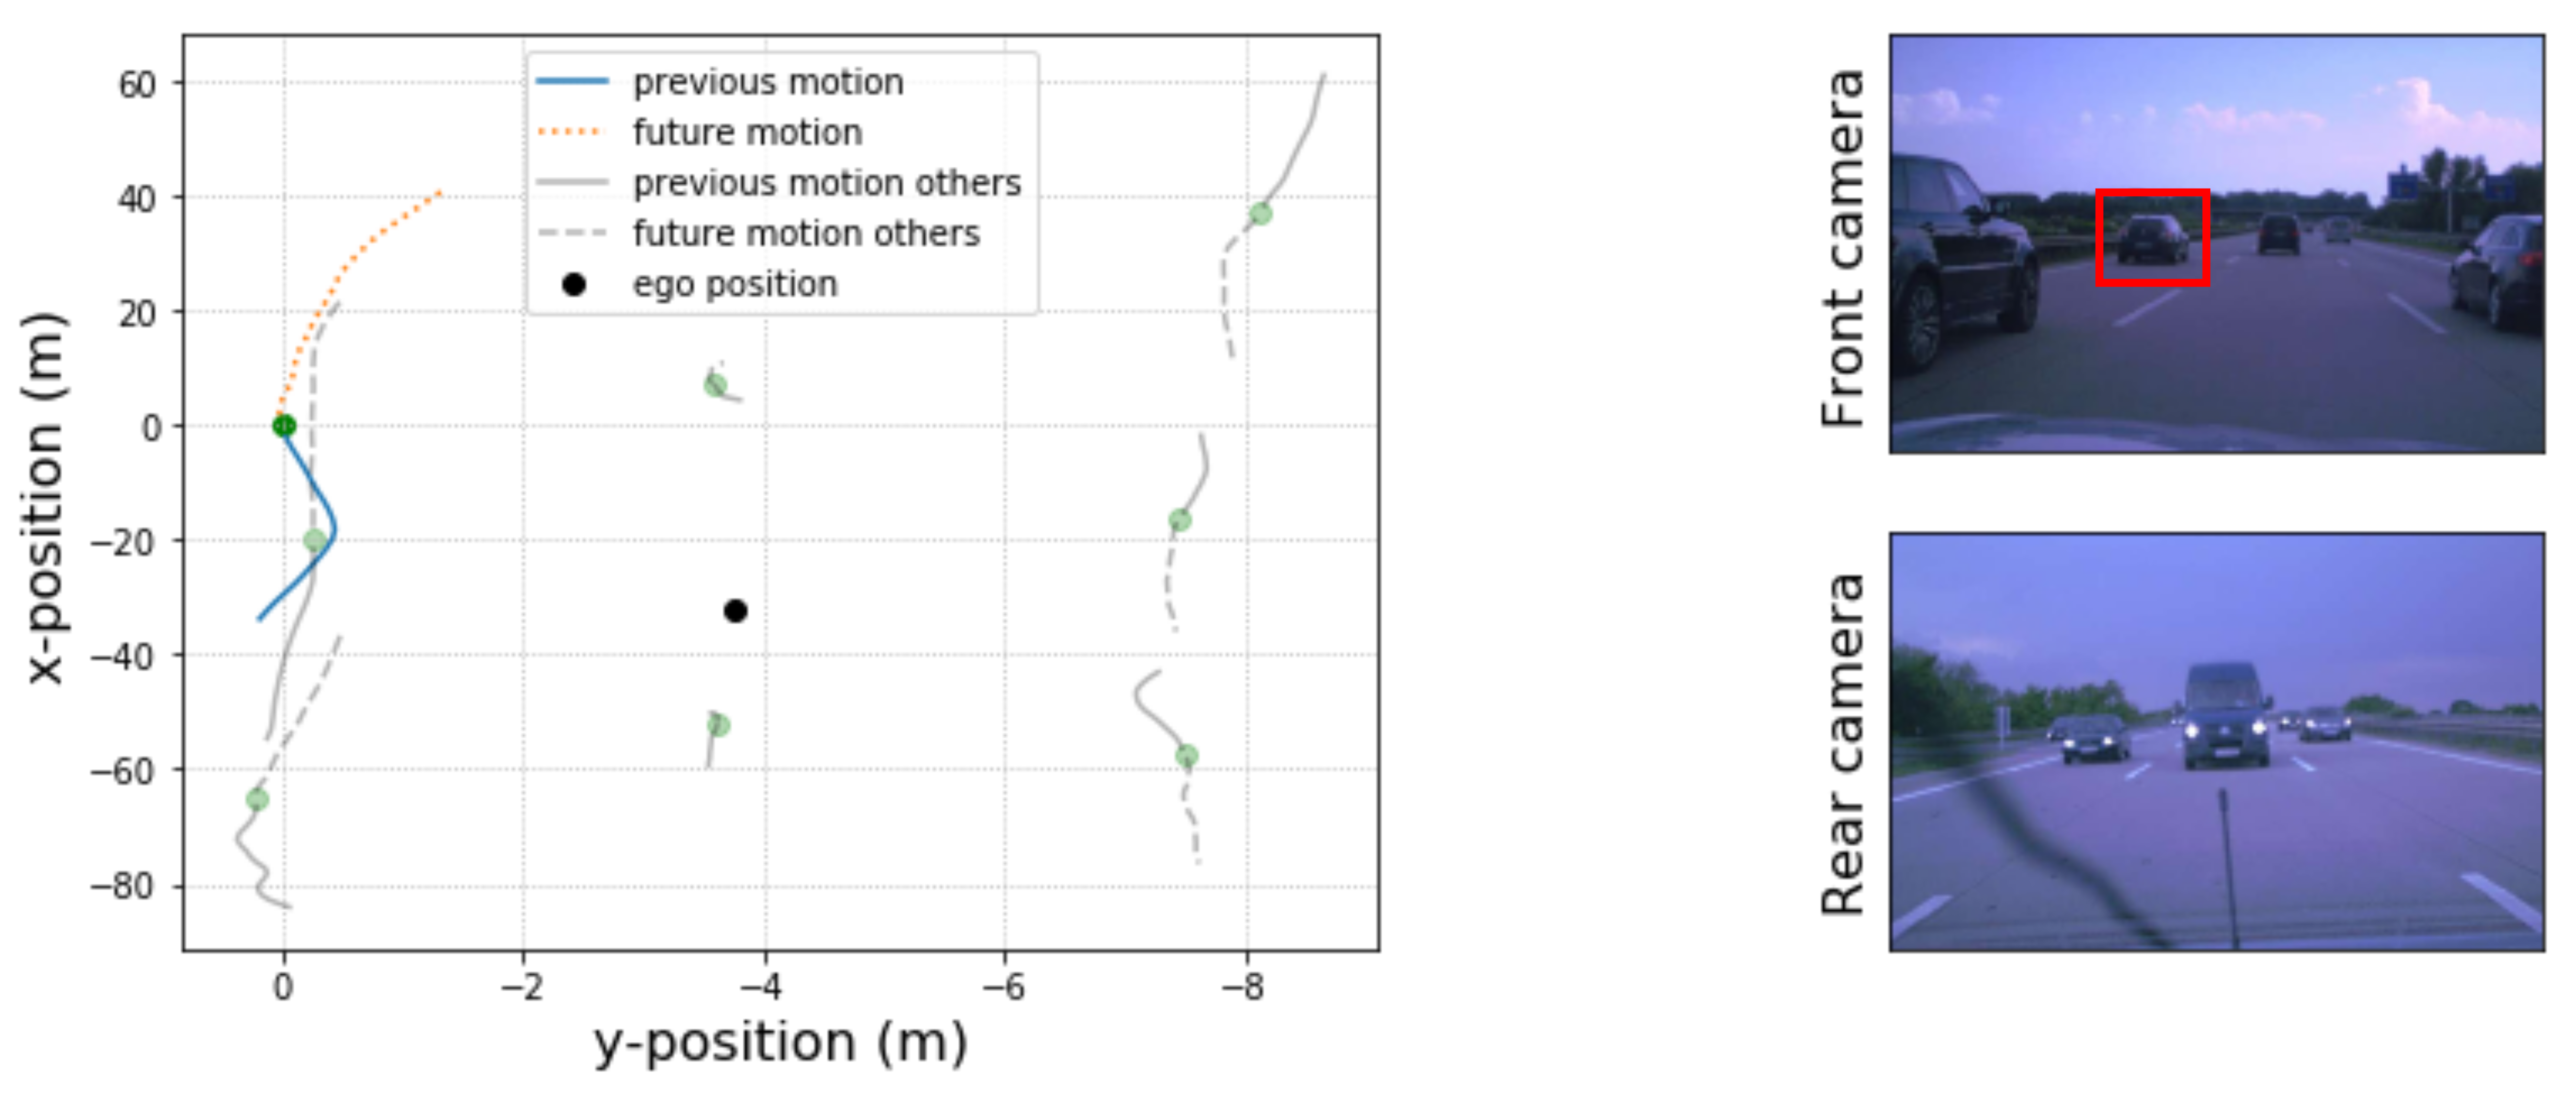
\includegraphics[width=\textwidth]{imgs/on_board_example_with_imgs_target.png}
    \caption{Data visualization of one driving situation example from the \emph{On-board} data-set $D_1$. The dots in the left plot indicate the position of the vehicles and color-code the vehicle type (red=motorcycle, green=car, blue=truck, black=ego-vehicle), blue and orange lines show past and future motion of the target vehicle whereas gray lines depict the other vehicles' motion. The right figures show raw images of the front and rear camera with the target vehicle
    highlighted by a red rectangle..}\label{fig:on_board_data_example}
\end{figure}

This is our main data-set used in this chapter.
It contains real-world data gathered using the vehicle's on-board sensors during test drives mainly on highways in southern Germany.
The data contains object-lists with a variety of features obtained from different sensor sources.
Apart from features about motion and behavior of the dynamic objects in the scene like position, velocity and acceleration, which are estimated from \ac{LIDAR} sensors, there is also visual information like object type probabilities or lane information, which is acquired from additional camera sensors (see \cite{Aeberhard2015} for further information on the sensor setup).
Table~\ref{tab:target_data_features} gives an overview and detailed description of the data features available in this data-set, which are relevant for our models.
\begin{center}
	\begin{tabular}{|l | p{12cm}|}
		\hline
		\textbf{Data label} & \textbf{Description}\\ \hline
		Position & Lateral/Longitudinal position absolute/relative to the ego vehicle's position estimated from range sensor readings \\ \hline
		Velocity& Lateral/Longitudinal velocity absolute/relative to the ego vehicle's velocity estimated from range sensor readings \\ \hline
		Acceleration & Lateral/Lateral acceleration absolute/relative to the ego vehicle's velocity estimated from range sensor readings \\ \hline
		Lane & Information about the lane relative to ego vehicle estimated from fused sensor reading (camera and range sensors) \\ \hline
		LaneBorderDistance & Distance to left/right border of the current lane estimated from fused sensor reading (camera and range sensors) \\ \hline
		LaneCurvature & Information about the lane curvature estimated from fused sensor reading (camera and range sensors) \\ \hline
		TypeProbability & Probability for the object being a of certain type (e.g. car or truck) estimated from camera sensors \\ \hline
	\end{tabular}
	\label{tab:target_data_features}
	\captionof{table}{Table depicting different features for dynamic objects within the training data}
\end{center}
The fused information about objects is available at a frequency of roughly \SI{5}{\hertz}.
The main feature of this data-set is that all information (position, velocity, etc.) about vehicles other than the ego-vehicle are measured with respect to that ego-vehicle and its coordinate system.
Fig. ~\ref{fig:on_board_data_example} shows one example situation from this data-set: the left plot depicts the positional information of all vehicles detected by the ego-vehicle's on-board sensors.
On the right-hand side, the raw images from the front and rear camera give an impression of the driving situation at hand with the target vehicle highlighted by a red box.
In total, the \emph{On-board} data-set contains \num{3891} vehicles, which yield a total length of roughly \SI{28.3}{\hour} when adding up the time each individual vehicle is visible.

\subsection{\acs{NGSIM} US-101 data-set}
\label{subsec:ngsim-dataset}

The \ac{NGSIM} US-101 data-set \cite{NGSIM-US101} is a publicly available data-set recorded on a segment of approximately \SI{640}{\meter} length with \num{6} lanes on the US-101 freeway in Los Angeles, California.
Although the data-set was originally intended for driver behavior and traffic flow models \cite{He2017}, it has also been used to train trajectory predictions models \cite{Altche2018, Deo2018}.
The data-set was recorded using cameras observing freeway traffic from rooftops with trajectory-data being extracted later from the obtained video footage.
Fig.~\ref{fig:ngsim_dataset} shows the recorded highway segment from top view perspective indicating the camera's position (fig.~\ref{subfig:ngsim_highway_top_view}) as well as the visualization of one example driving situation (fig.~\ref{subfig:ngsim_example_xy}).
The data-set holds a total of \SI{45}{\minute} of driving data split into three \SI{15}{\minute} segments of mild, moderate and congesting traffic conditions.
Apart from positional information in lateral and longitudinal direction (in a global and local coordinate system), additional features like instantaneous velocity, acceleration, vehicle size as well as the current lane are available for each vehicle.
The trajectory data is sampled with a frequency of \SI{10}{\hertz}.
The main difference to the \emph{On-board} data-set is the fact, that the \emph{\ac{NGSIM}} data-set is recorded with external stationary cameras instead of a driving vehicle's on-board sensors.
\begin{figure}[t!]
	\centering
	\resizebox{.95\textwidth}{!}{%
		\subfloat[\label{subfig:ngsim_highway_top_view}]{%
			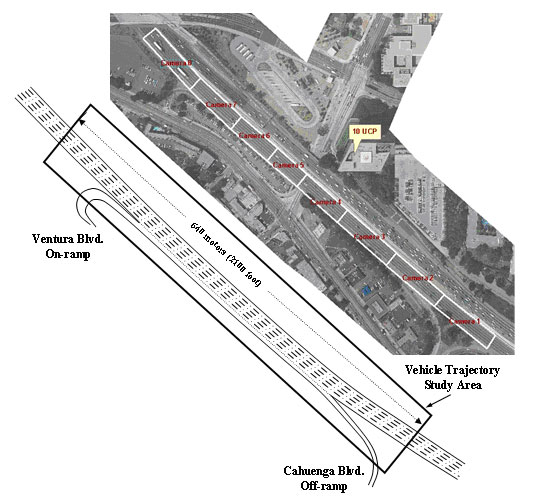
\includegraphics[height=4cm]{imgs/ngsim_highway_top_view.jpg}
		}
		\subfloat[\label{subfig:ngsim_example_xy}]{%
			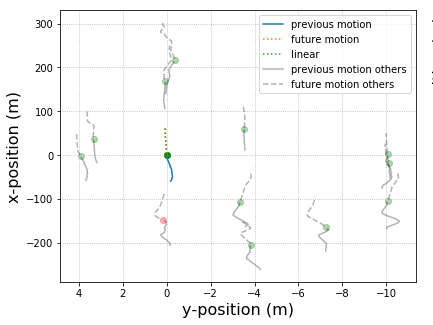
\includegraphics[height=4cm]{imgs/ngsim_example_xy.png}
		}
	}
    \caption{Visualization of \emph{\ac{NGSIM}} data set: ~\protect\subref{subfig:ngsim_highway_top_view} depicts the highway segment from top view perspective indicating the camera's position (source \cite{NGSIM-US101}) ~\protect\subref{subfig:ngsim_example_xy} visualizes the data of one particular driving situation from the data-set.}\label{fig:ngsim_dataset}
\end{figure}
Thus, there is no ego-vehicle present in the data and all information are available in absolute coordinates instead of being measured relative to one particular ego-vehicle.
In total, the \emph{\ac{NGSIM}} data-set contains \num{5930} vehicles and therefore a total time of roughly \SI{91.3}{\hour} when adding up the time each individual vehicle is visible.

\subsection{Preprocessing}
\label{subsec:preproc}

In this section, we describe the preprocessing steps performed a priori to prepare the information from our two data-sets as neural network input.
Although we aim to keep these preprocessing steps as consistent as possible across the data-sets, there are some mild differences, which we will also point out.
We aim to predict future positions of dynamic objects \SI{5}{\second} into the future based on their positions \SI{5}{\second} prior to their current location one object at a time.
As the two data-sets are sampled at different frequencies, we interpolate the available data over 20 equidistant steps to achieve intervals of \SI{0.25}{\second} to improve consistency and comparability.
Furthermore, we translate the current position of the target vehicle (the vehicle to be predicted) into the origin, i.e. position $\left(0,0\right)$ (see Fig.~\ref{fig:data_example}), to prevent our models from treating similar trajectories differently due to positional variations.
Finally, to improve suitability of the data as input for neural networks, we divide all $x$-positions by a factor of \num{10} such that $x$-/$y$-values are scaled to a similar order of magnitude.
For the \emph{\acs{NGSIM}} data-set $D_2$, we use only every \num{10}th data point, to avoid the creation of too many overlapping, and therefore too similar, data samples.
Furthermore, we swapped the dimensions of the positions in $D_2$ such that for both data-sets $x$- and $y$-direction correspond to longitudinal and lateral positions respectively.
For training and evaluating our models, we split both data-sets into training $T_i \subset D_i$ and validation data $V_i \subset D_i$ containing \SI{90}{\percent} and \SI{10}{\percent} of the objects respectively with $T_i \cap V_i = \varnothing$ to avoid testing our models on vehicles they have been trained with.

\subsection{Data peculiarities}
\todo[inline]{mention and analyze the composition of the data-set with mainly straight driving and particular interesting situations occurring rather rarely}

\subsection{Performance baselines}
\label{subsec:baselines}
\todo[inline]{Formulation: In this section, we analyze!}
Figure~\ref{fig:overtaking} shows an example of an overtaking maneuvre in a highway situation.
The ego-vehicle is overtaken by another car approaching from behind.
Subfigures~\ref{subfig:overtaking1}--~\ref{subfig:overtaking4} show different times of the maneuvre.
Solid lines indicate previous positions whereas dashed lines indicate future positions or predictions.
The dashed green line illustrates linear predicions based on a constant velocity assumption for $x$ direction and linear regression using the last \SI{0.5}{\second} of the positions for $y$ direction.
\begin{figure}[H]
	\centering
	\subfloat[Overtaking maneuvre at $t=\SI{90}{\second}$\label{subfig:overtaking1}]{%
		\includegraphics[clip,width=\columnwidth]{imgs/Vis_overtaking_maneuvre_t1.png}
	}
	\vspace{-0.3cm}
	\subfloat[Overtaking maneuvre at $t=\SI{94}{\second}$\label{subfig:overtaking2}]{%
		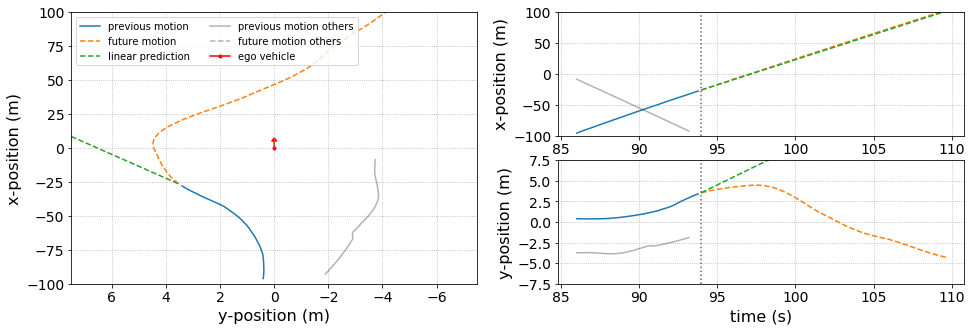
\includegraphics[width=\columnwidth]{imgs/Vis_overtaking_maneuvre_t2.png}
	}
	\vspace{-0.3cm}
	\subfloat[Overtaking maneuvre at $t=\SI{98}{\second}$\label{subfig:overtaking3}]{%
			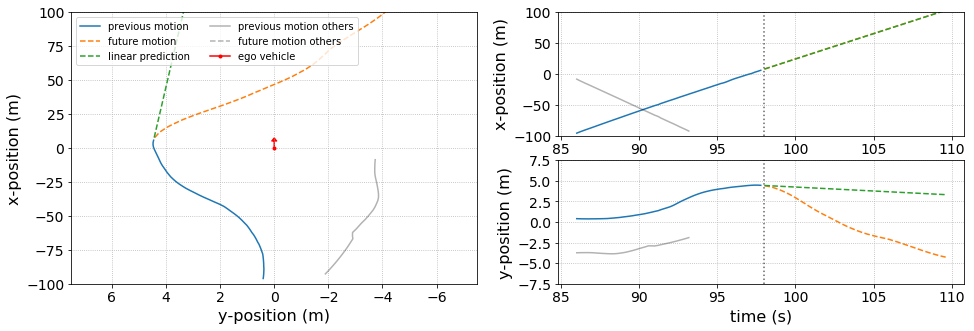
\includegraphics[width=\columnwidth]{imgs/Vis_overtaking_maneuvre_t3.png}
	}
	\vspace{-0.3cm}
	\subfloat[Overtaking maneuvre at $t=\SI{100}{\second}$\label{subfig:overtaking4}]{%
			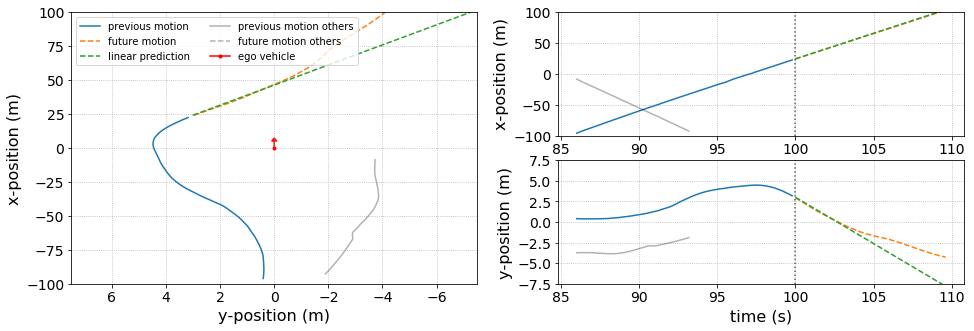
\includegraphics[width=\columnwidth]{imgs/Vis_overtaking_maneuvre_t4.png}
	}
	\caption{An example scene visualizing the data of an overtaking maneuver in a highway situation at selected time steps.} \label{fig:overtaking}
\end{figure}

\begin{itemize}
	\item linear regression
	\item kalman filters?
	\item traditional neural networks (\ac{NEF} networks and \ac{LSTM} networks)
	\item something else?
\end{itemize}

\section{Representation and models}
\label{sec:repr_models}

In this section, we describe our approach of how to encode spatial information of driving situations in semantic vectors of fixed length.
Therefore, we use the convolutive vector power introduced in def.~\ref{def:conv_power}.
For reference, we also describe a simpler vector representation as well as a raw numerical representation encoding only the positional information of the target vehicle.  
Furthermore, we describe the architecture of the learning models used for behavior prediction from that input data.
Importantly, here we use our models to predict one particular target vehicle at a time instead of trying to jointly predict the progress of the entire scene.
To achieve a forecast of the development of all vehicles in the scene, we would deploy several instantiations of the same network.
Using this approach, we only have to train one model while we can use each detected vehicle as training example, which increases the amount of our training data. 


\subsection{Scene representation in vectors}
\label{subsec:scene_repr}
\begin{figure}[t!]
  \centering
  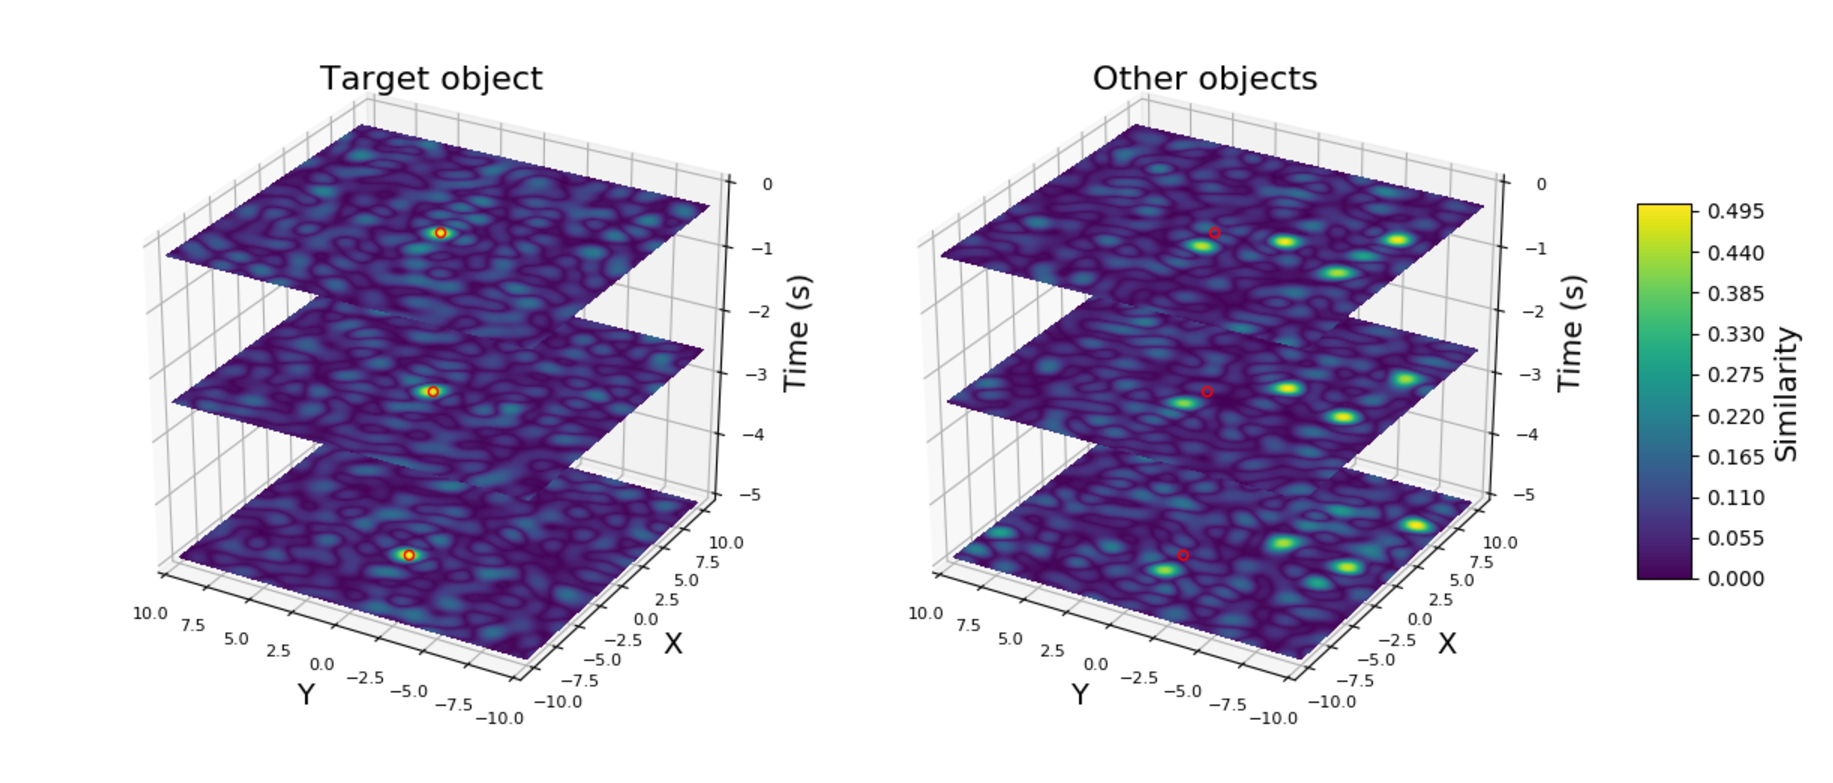
\includegraphics[width=0.95\textwidth]{imgs/spa_power_representation_in_time_viridis.eps}
  \caption{Visualization of the convolutive vector-power representation of one particular driving situation over time at selected time-steps as a heat map of similarity values for \num{512}-dimensional vectors. The red circles indicate the measured position of the target vehicle.}\label{fig:spa_power}
\end{figure}

In this section, we investigate the expressive power of encoding the spatial positions of multiple vehicles using the convolutive vector-power introduced in def.~\ref{def:conv_power}.
To create a vocabulary $V$ of atomic vectors, we assign a random real-valued vector from the unit sphere to each category of dynamic objects (e.g. car, motorcycle, truck) as well as random unitary vectors (c.f.\ def. ~\ref{def:unitary_vec}) $\mathbf{X}$ and $\mathbf{Y}$ to encode spatial positions.
We use unitary vectors for $\mathbf{X}$ and $\mathbf{Y}$ as they have unit length and are closed under convolutive exponentiation.
Therefore, by encoding spatial positions with powers of unitary vectors, we avoid exploding lengths of our final scene vectors, which would lead to additional noise and unwanted behavior when using them as input for neural networks.
Furthermore, we use additional random ID-vectors $\mathbf{TARGET}$ and $\mathbf{EGO}$ representing the target object to be predicted and, if applicable, the ego-vehicle.
Given a situation as shown in Fig.~\ref{fig:data_example} \textbf{(A)} with a sequence of prior positions $(x_{t}, y_{t})$ for the target vehicle at time step $t \in \left\{t_{0}, \ldots, t_{N} \right\}$ and equivalent sequences $(x_{obj,t}, y_{obj,t})$ for other traffic participants, we encapsulate this information in a scene vector

\begin{equation}
	\label{eq:conv_power_enc}
  \mathbf{S}_{t} = \underbrace{\mathbf{TARGET}\varoast \mathbf{TYPE}_{target} \varoast \mathbf{X}^{x_{t}} \varoast \mathbf{Y}^{y_{t}}}_{\textrm{target-vehicle}} \oplus \underbrace{\sum_{obj} \mathbf{TYPE}_{obj} \varoast \mathbf{X}^{x_{obj,t}} \varoast \mathbf{Y}^{y_{obj,t}}}_{\textrm{other objects}},
\end{equation}
This yields a sequence of semantic scene vectors $\mathbf{S}_{t}$ for $t \in \left\{t_{0}, \ldots, t_{N} \right\}$ encoding the past spatial development of objects in the current driving situation.
Fig.~\ref{fig:spa_power} depicts the aforementioned scene vector representation: the left plots show similarities (depicted as heat map) between the vector $\mathbf{S}_{t}$ encoding the scene from Fig.~\ref{fig:data_example} \textbf{(A)} and the vectors $v_{i}=\mathbf{TARGET}\varoast \mathbf{TYPE}_{target} \varoast \mathbf{X}^{\bar{x}_{i}} \varoast \mathbf{Y}^{\bar{y}_{i}}$ for a sequence of discrete position samples ${\bar{x}_{i}, \bar{y}_{i}}$.
Similarly, the right plots show similarities between $\mathbf{S}_{t}$ and $\mathbf{CAR} \varoast \mathbf{X}^{\bar{x}_{i}} \varoast \mathbf{Y}^{\bar{y}_{i}}$ visualizing all other objects in the scene of type \emph{car}.
Hence, we can encode spatial information of several different objects in a sequence of semantic vectors and reliably decode it back out.
This allows us to encode automotive scenes with varying number of dynamic objects in a vector representation of fixed dimensionality.
Note that by using this vector representation as input data for a neural network (or any other predictor), we predict the future position of one other traffic participant at a time.
The indication vector $\mathbf{TARGET}$ bound to the object we want to predict indicates the network the current focus.
To predict all objects present in a scene during deployment, multiple instantiations of the same network can be used.
Thereby, the amount of training data generated per file increases with the number of objects while we only need to train one network.

\subsection{Prediction models}
\label{subsec:pred_models}
\begin{figure}[t!]
  \centering
  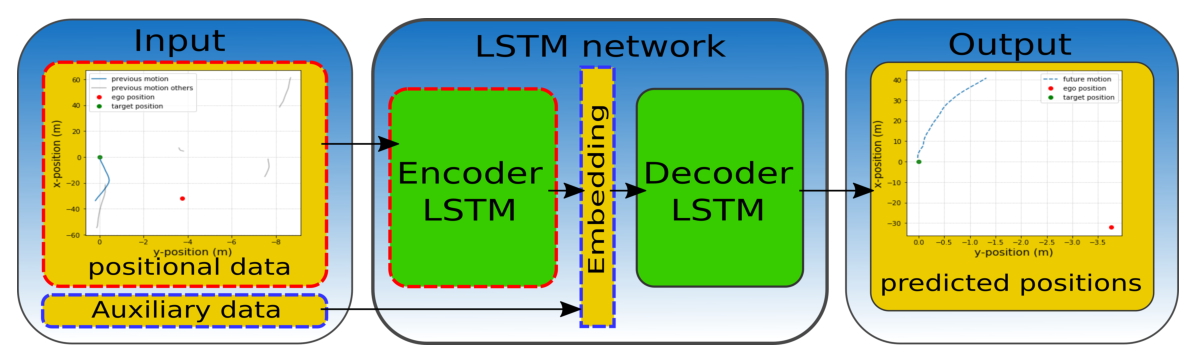
\includegraphics[width=0.95\textwidth]{imgs/lstm_arch.eps}
  \caption{Visualization of our \ac{LSTM}-based learning architecture. Modules that change with varying encoding scheme of the input data are highlighted through dashed red borders whereas parts that change when varying the data-set are highlighted through dashed blue borders.}\label{fig:lstm_arch}
\end{figure}


In this section, we describe the models we use for the behavior prediction task.
The input data for our models are sequences of positional data either as raw numerical values or in the form of semantic vectors as described in sec. ~\ref{subsec:scene_repr}.
\ac{LSTM} neural network architectures have proven to be powerful tools for sequential data analysis and are widely used for behavior, or more generally, motion prediction.
We also investigate much simpler feed-forward neural networks constructed using the principles of the \acl{NEF} (c.f.~\ref{sec:neural_eng}) to evaluate the performance gains achieved by the more complex \ac{LSTM} models.

\subsubsection{\acs{LSTM} networks}
\label{subsubsec:lstm_models}
In this work, we use a \acf{LSTM} \cite{Hochreiter1997} network-architecture for the prediction of vehicle positions.
Our network consists of one \ac{LSTM} encoder and decoder cell for sequence to sequence prediction, which means that the input and the final result of our model is sequential data.
The encoder \ac{LSTM} takes positional data for $20$ past, equidistant time frames as input.
The resulting embedding vector encodes the history of the input data over those time frames.
This embedding vector is concatenated with additional auxiliary information to aid the model when predicting the future trajectory of the target vehicle.
This auxiliary data should be information, that is available to the system when the prediction is to happen (see Sec.~\ref{subsubsec:train_lstm} for further details on this auxiliary data).
Finally, the embedding vector is used as input for the decoder \ac{LSTM} to predict future vehicle positions.
We use the same network architecture for all encoding schemes of the input data and for both data-sets.
However, the dimensionality of the input and the information used as auxiliary information to enrich the embedding vector vary over different encoding schemes and data-sets respectively (see Sec.~\ref{subsubsec:train_lstm} for details).
Fig.~\ref{fig:lstm_arch} visualizes the architecture of our \ac{LSTM} models indicating modules that change when varying the encoding scheme by a dashed red border whereas parts that change with the data-set are highlighted through a dashed blue border.

\subsubsection{\acs{NEF} networks}
\label{subsubsec:nef_models}

As an alternative to the \ac{LSTM}-models, we also considered a much simpler single-hidden-layer network defined using the Neural Engineering Framework (\ac{NEF}) \cite{Eliasmith2003}.
While this is usually used for constructing large-scale biologically realistic neuron models \cite{Eliasmith2012}, the \ac{NEF} software toolkit \acs{Nengo} \cite{Bekolay2014} also allows for traditional feed-forward artificial neural networks using either spiking or non-spiking neurons.
For these \ac{NEF} networks, we use a single hidden layer, with randomly generated (and fixed) input weights, and use least-squares optimization to compute the output weights.
As with any traditional network, we can have any number of input, output, and hidden neurons, all following this same process.
The goal here is to provide a simple baseline for comparison to the \ac{LSTM} networks, to see what (if any) performance gain is produced by the more complex network approach.
However, these simpler networks are unable to process sequential data in the same way as the \ac{LSTM} models.
Therefore, we will have to slightly adapt our data, especially the semantic vector sequences, to make it suitable as input for the feed-forward networks.

\section{Experiments and results}
\label{sec:experiments}
In this section, we describe the training process and parameters of all our models and give a detailed analysis and evaluation of the results achieved.
The \ac{LSTM} models are implemented in Tensorflow \cite{Abadi2016} whereas the \ac{NEF} models and the mixture-of-experts online learning model are implemented using the \acs{Nengo} software suite \cite{Bekolay2014}.
We use the \ac{RMSE} as our main metric for evaluation purposes.
In contrast to earlier work, we inspect the \ac{RMSE} for lateral and longitudinal directions separately to give more detailed insights into the models' behavior.
Furthermore, we investigate where the models shows their best performance looking for correlations between prediction accuracy and specific driving situations.

\subsection{Hyperparameter analysis}
\label{subsec:hyperparam_analysis}
Before we proceed to compare and evaluate our models using each available encoding scheme, we aim to find a suitable set of hyperparameters.
Therefore, we conduct a thorough analysis on both our network architectures using only numerical input data for simplicity and to keep the time needed for training limited.
Systematically, we only analyze one parameter at a time and fix the best value for that parameter for the subsequent analysis of other parameters.
However, we also inspect certain parameter pairs jointly if there are correlations or mutual influences between the parameters to be expected.

\subsubsection{\ac{LSTM} networks}
\label{subsubsec:hyperparam_lstm}

\begin{figure}[t!]
  \centering
  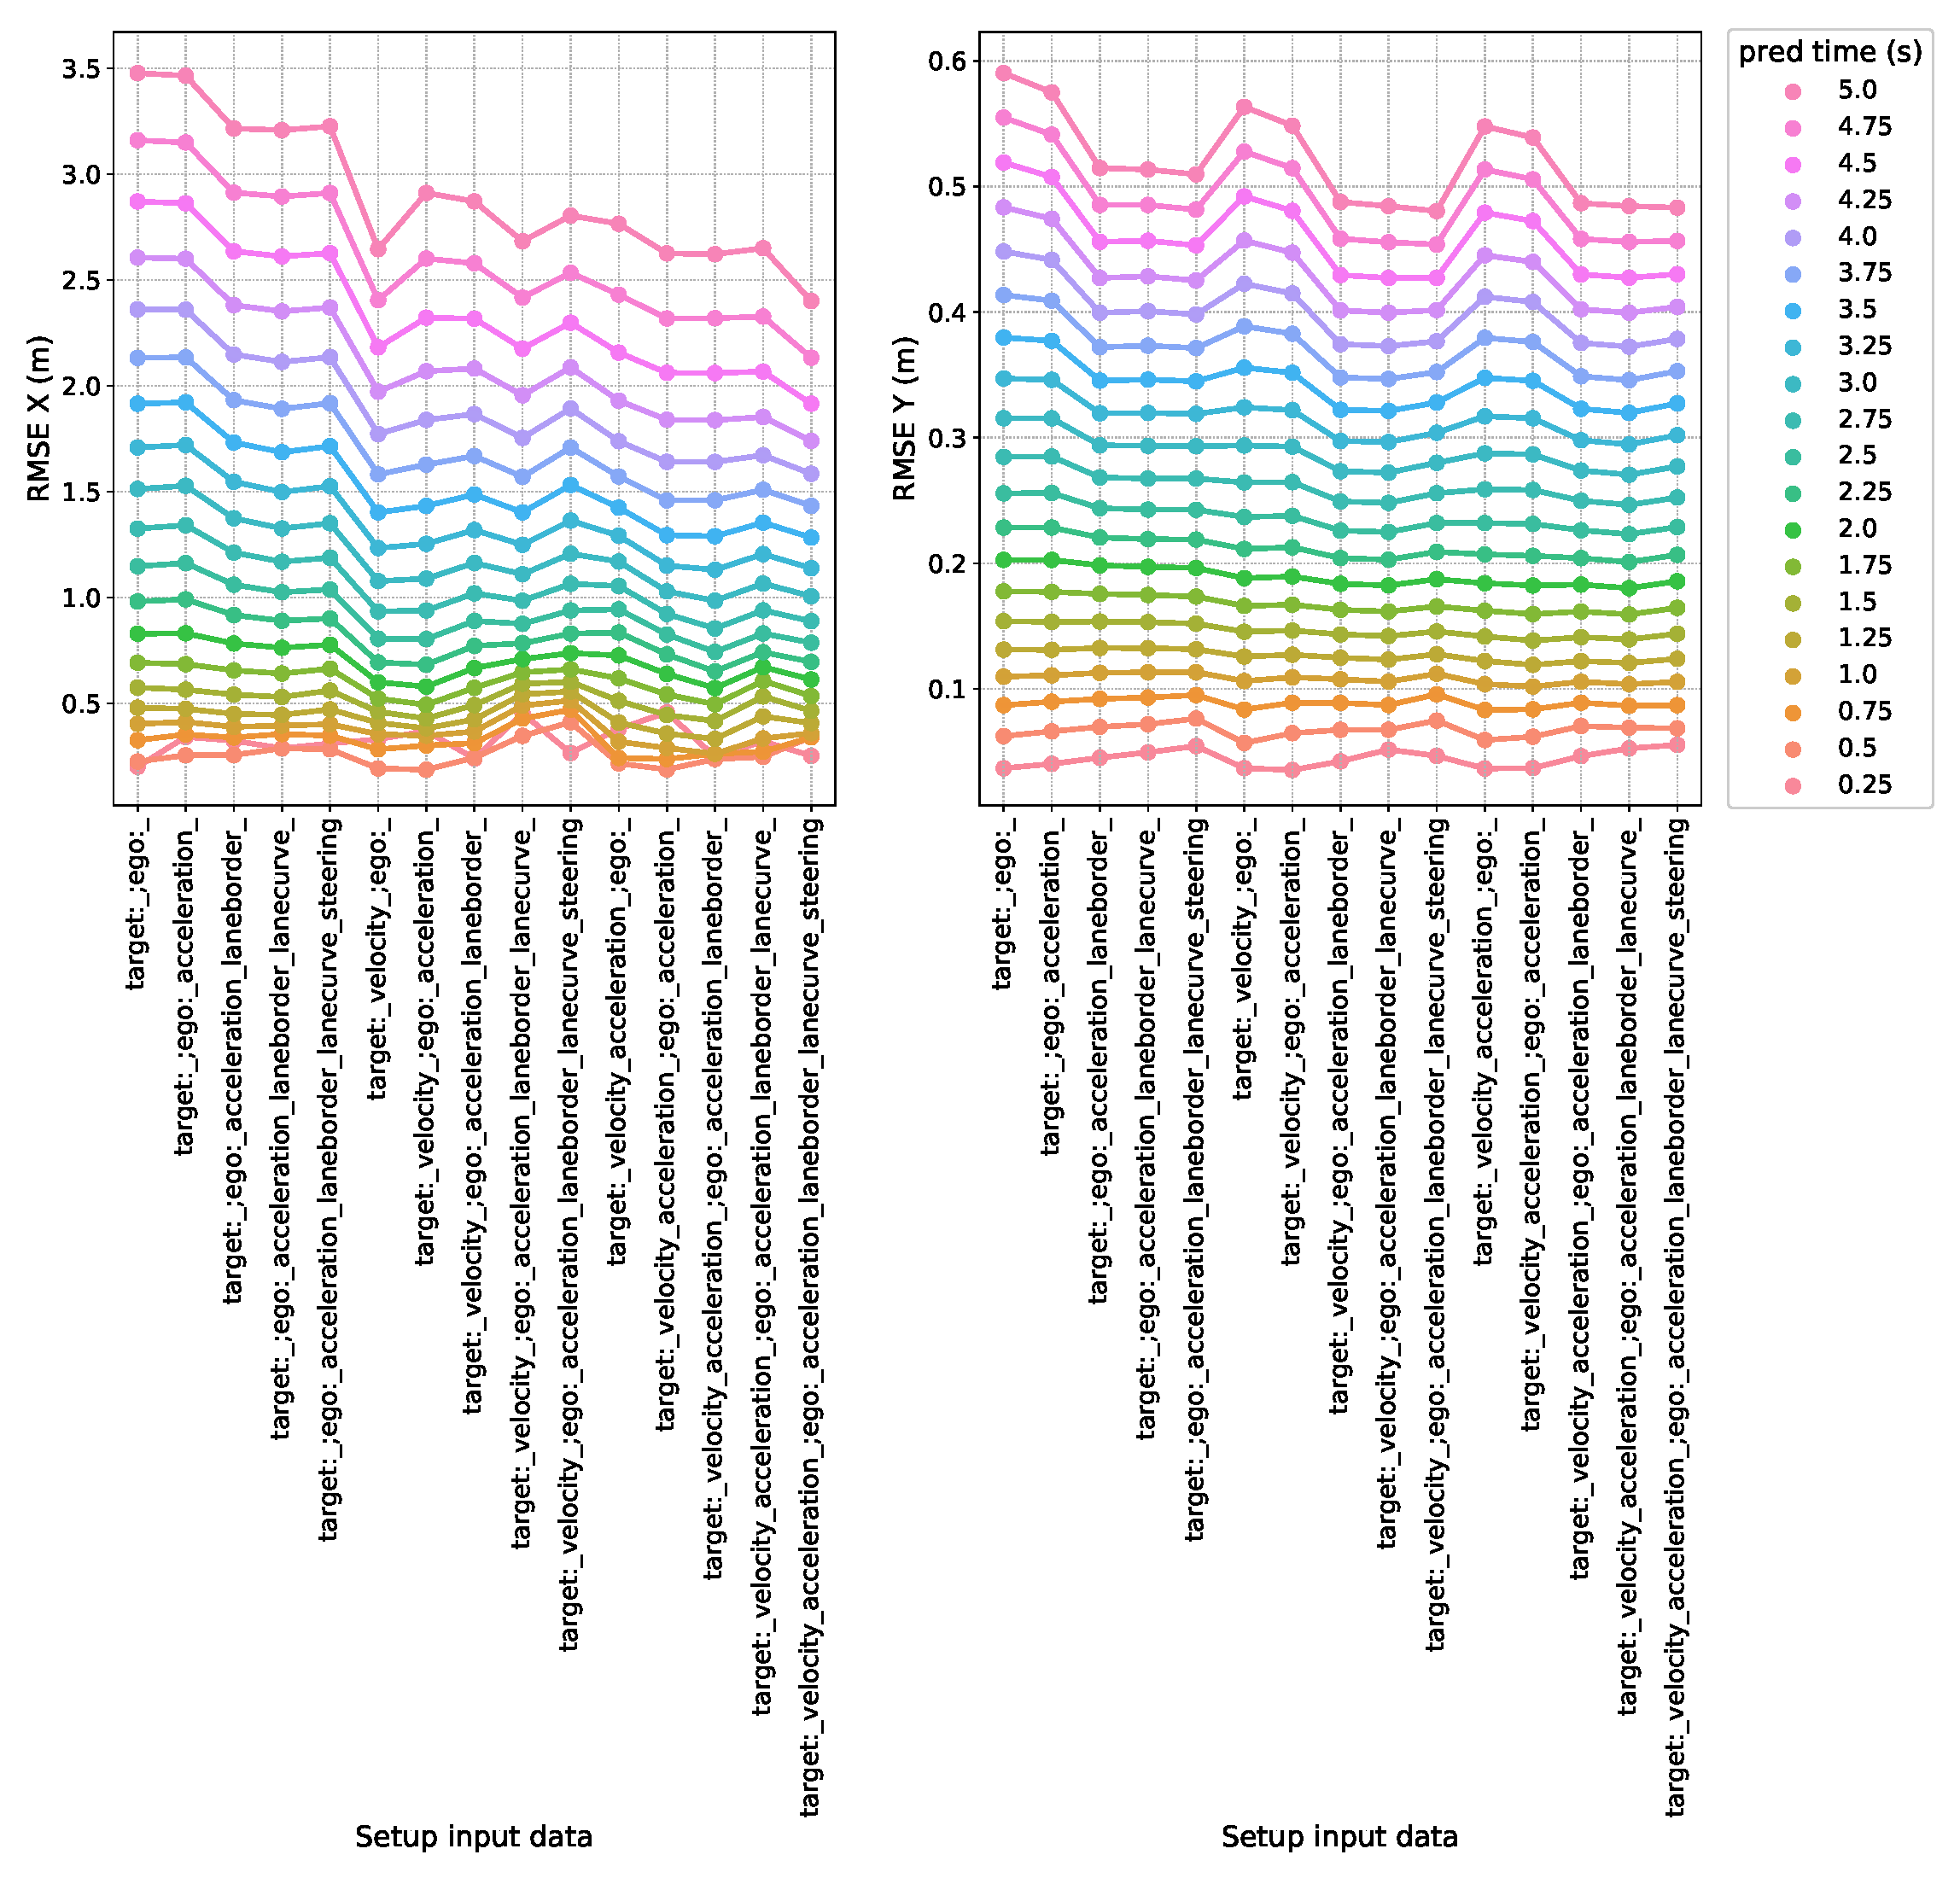
\includegraphics[width=0.95\textwidth]{imgs/lstm_input_data_analysis.eps}
  \caption{Analysis of the \ac{RMSE} for different variations of numerical input to our \ac{LSTM} model trained on the \emph{On-board} data-set for \num{8} epochs.}\label{fig:lstm_input_data_analysis}
\end{figure}

For the \ac{LSTM}-models, we firstly investigated the composition of the input data to the model to get an idea, what kind of information is useful for the task of motion prediction.
Therefore, we trained several instantiations of our \ac{LSTM}-network architecture as described in Sec.~\ref{subsubsec:lstm_models} on the \emph{On-board} data-set $D_1$ for different variations of the input data, for \num{8} epochs each.
The simplest setting is using only the positional information of the target vehicle as input and its instantaneous velocity as additional information in the embedding without including any information about the ego-vehicle.
We refer to this setting as the default setting in this section.
In addition, we also analyze settings where additional information like velocity and acceleration of the target vehicle are available to the system.
Furthermore, if all dynamic information are available relative to the ego-vehicle, there are other features that could be useful for motion prediction such as the current curvature of the road or the current velocity or steering values of the ego-vehicle itself.
For example, if the ego-vehicle performs a lane change or the road bends, this will influence the relative motion of all other vehicles while this information most likely will not be available from just the positions of the target vehicle. 
On the other hand, if such information is available to the system, it would improve the models capability of abstracting and inferring correlations between the available information in such situations.
In this evaluation, we include the history of the ego-vehicle's information to the input data and future values to the embedding, whereas we include additional information about the target vehicle to the input data only. 
\\
Fig.~\ref{fig:lstm_input_data_analysis} depicts the \ac{RMSE} ($y$-axis) for each input data setup ($x$-axis) at each prediction time step.
Each tick on the $x$-axis corresponds to one input setup, whereas each group of \num{5} ticks from left to right correspond to one fixed setup for the target vehicle.
The left group contains only the default data about the target vehicle, the middle group contains the history of the target vehicle's velocity and the right group contains additionally the history of the target vehicle's acceleration.
The ticks within one group correspond to one setting for the ego-vehicle, whereas again from left to right the amount of available information increases.
Therefore, the rightmost tick contains information about the ego-vehicles acceleration, distance to the lane border as well as the curvature of the current lane and its current steering values (information is added in this order from left to right). 
In other words, the further we go from left to right on the $x$-axis in fig~\ref{fig:lstm_input_data_analysis}, the more information is available to the system.
We observe that adding more information about both, the ego- and target-vehicle, indeed improves prediction accuracy significantly: the difference between the best and worst setting is more than \SI{1}{\meter} in $x$-direction and more than \SI{0.1}{\meter} in $y$-direction.
For both dimensions, the setting using all available information outperforms the simpler setups.
However, there are some interesting peculiarities visible in this analysis that are worth noting.
For instance, the input information improving performance in $x$-direction the most appears to be the target vehicle's velocity. 
Furthermore, the target vehicle's acceleration does not yield further significant improvements given its velocity is available.
Interestingly, the setting using only the target vehicle's velocity as additional information is closely behind the best setting in $x$-direction.
Furthermore, the performance boost of the setting using all available information (the rightmost tick) over the prior setting comes from the ego-vehicle's steering, which only appears when its acceleration information is also available.
For the $y$-direction we observe similar trends in that the target vehicle's acceleration does not yield significant improvements over its velocity.
However, here the information about the ego-vehicle's distance to the lane borders appears to be the input that gives the most significant improvements in $y$-direction.
That makes sense, as these inputs encode information about the ego-vehicle's motion in $y$-direction such as lane changes.
As the setting using all available information (the rightmost tick in fig.~\ref{fig:lstm_input_data_analysis}) is by far outperforming all other settings in $x$-direction and is on par with the best in $y$-direction, we use this data-setup for further analyzing the hyperparameters of the \ac{LSTM}-model.
\\
We continue our hyperparameter analysis by inspecting the number of units within the \ac{LSTM} cells.
\begin{figure}[t!]
	\centering
    \subfloat[\label{subfig:lstm_units_analysis}]{%
        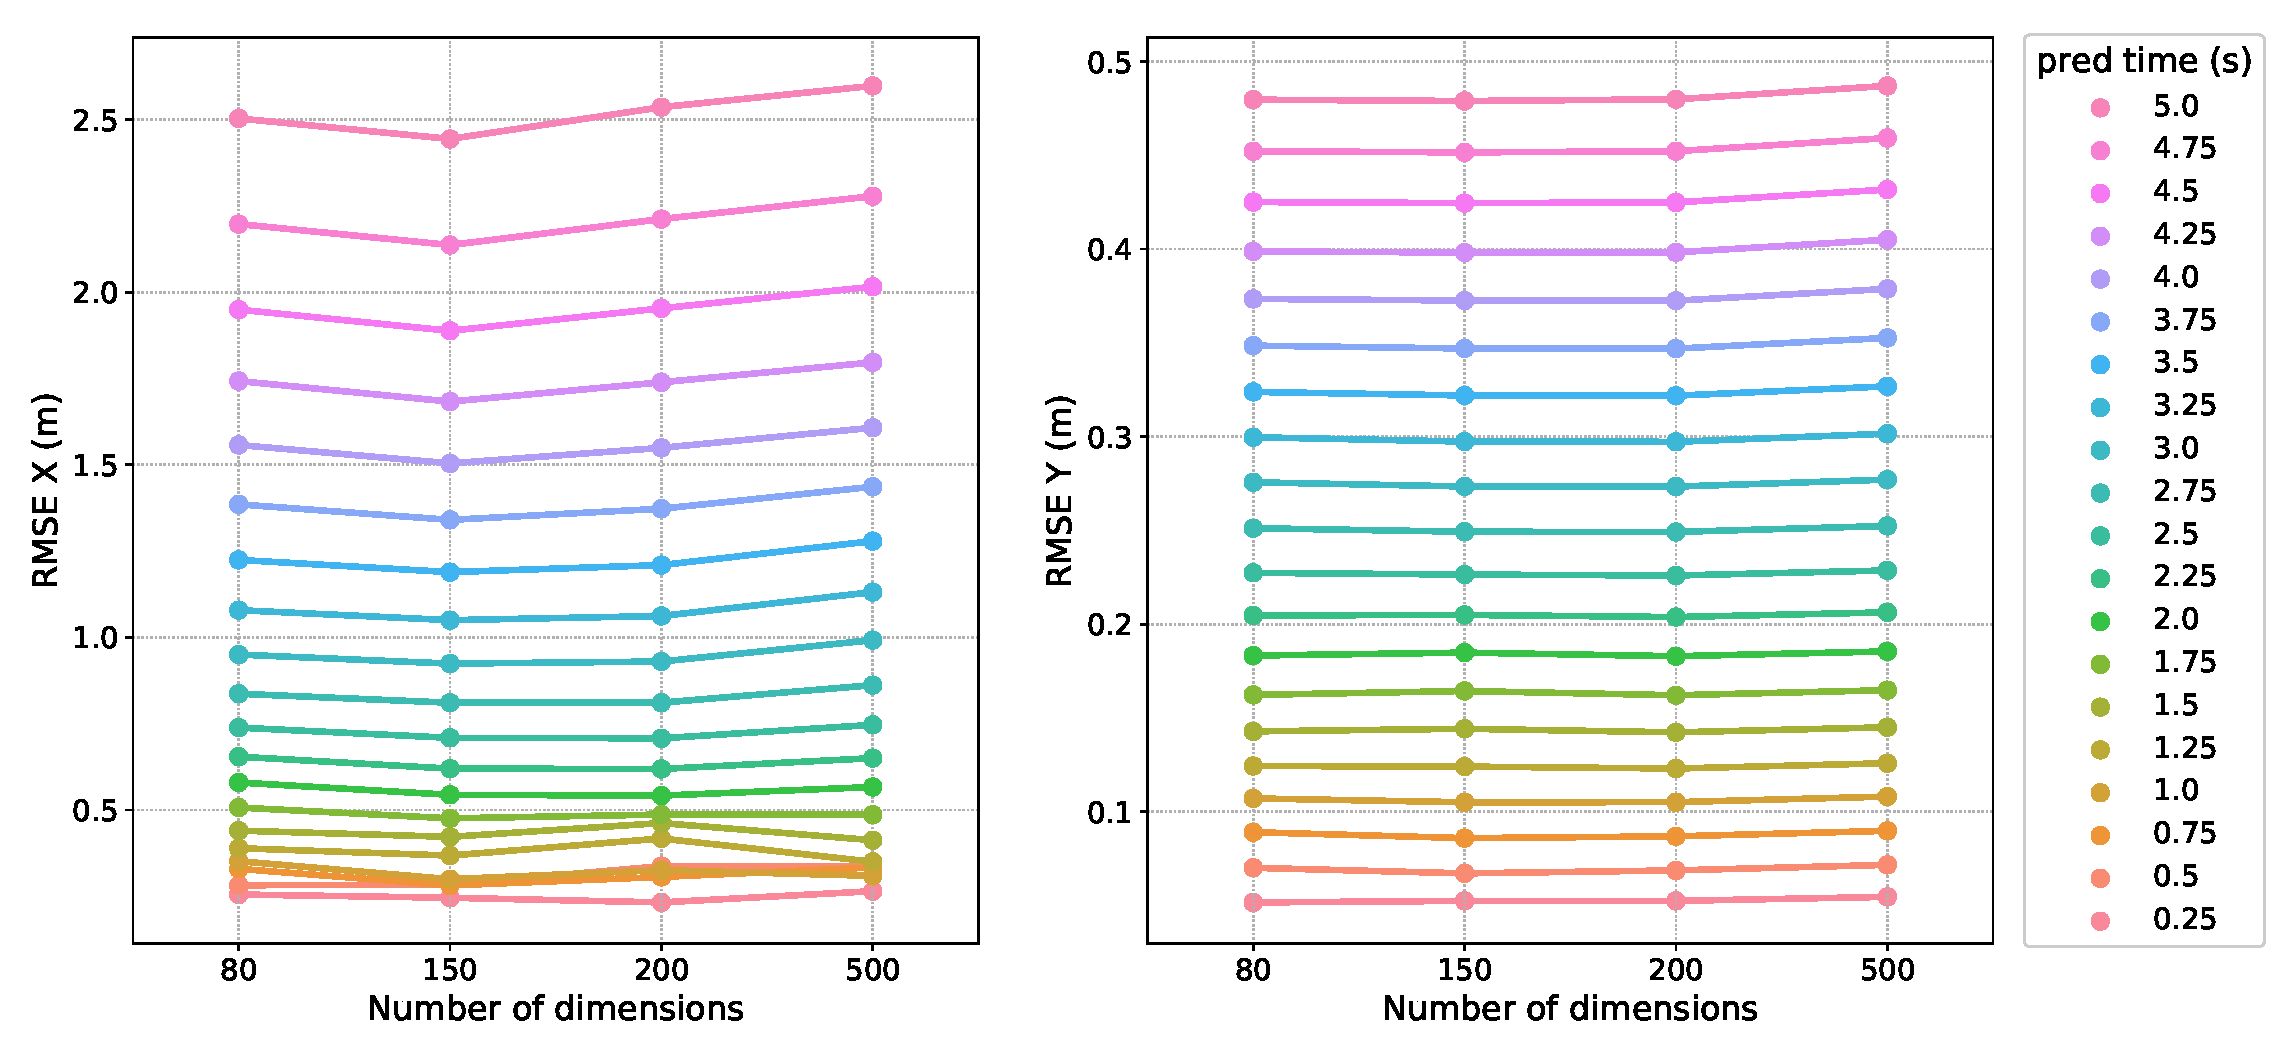
\includegraphics[width=\columnwidth]{imgs/lstm_units_analysis.eps}
    }
    \vspace{-0.3cm}
    \subfloat[\label{subfig:lstm_layers_analysis}]{%
        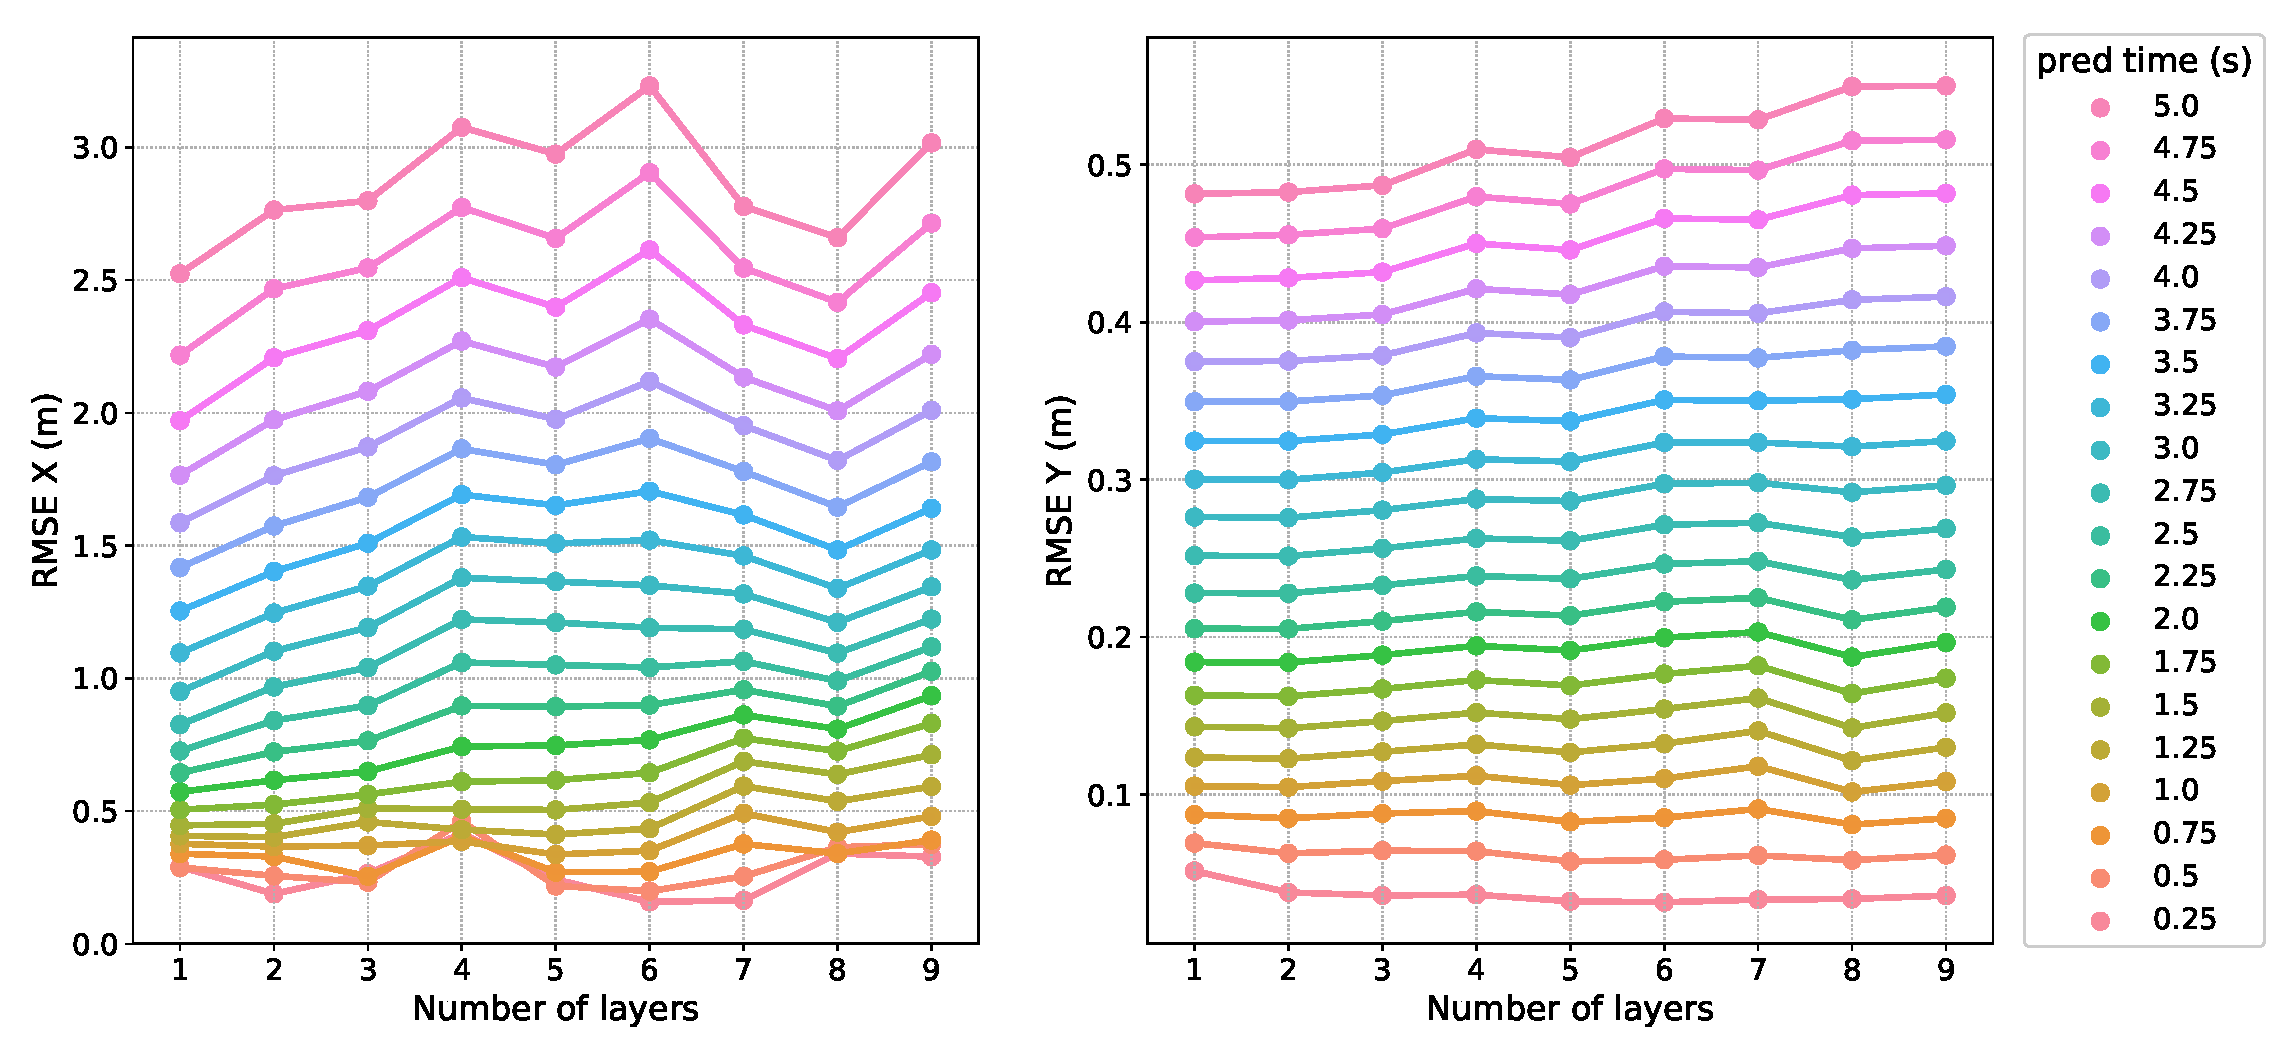
\includegraphics[width=\columnwidth]{imgs/lstm_layers_analysis.eps}
    }
    \caption{Visualization of the \ac{RMSE} for different parameter tests of our \ac{LSTM}-model trained on the \emph{On-board} data-set for \num{8} epochs:~\protect\subref{subfig:lstm_units_analysis} depicts the \ac{RMSE} when varying the number of units in each \ac{LSTM} cell~\protect\subref{subfig:lstm_layers_analysis} visualizes the \ac{RMSE} when varying the number of layers, i.e.\ the number of encoder and decoder \ac{LSTM} cells are used in the network.}
    \label{fig:ngsim_dataset}
\end{figure}
In our initial experiment, we used \num{80} units in each of the \ac{LSTM} encoder and decoder cell.
Here, we investigate if additional unit improve the models' prediction performance.
Again, we train the model for \num{8} epochs.
Fig.~\ref{subfig:lstm_units_analysis} depicts the \ac{RMSE} for a models with \num{80}, \num{150}, \num{200} and \num{500} units in the \ac{LSTM} cells.
\begin{figure}[t!]
  \centering
  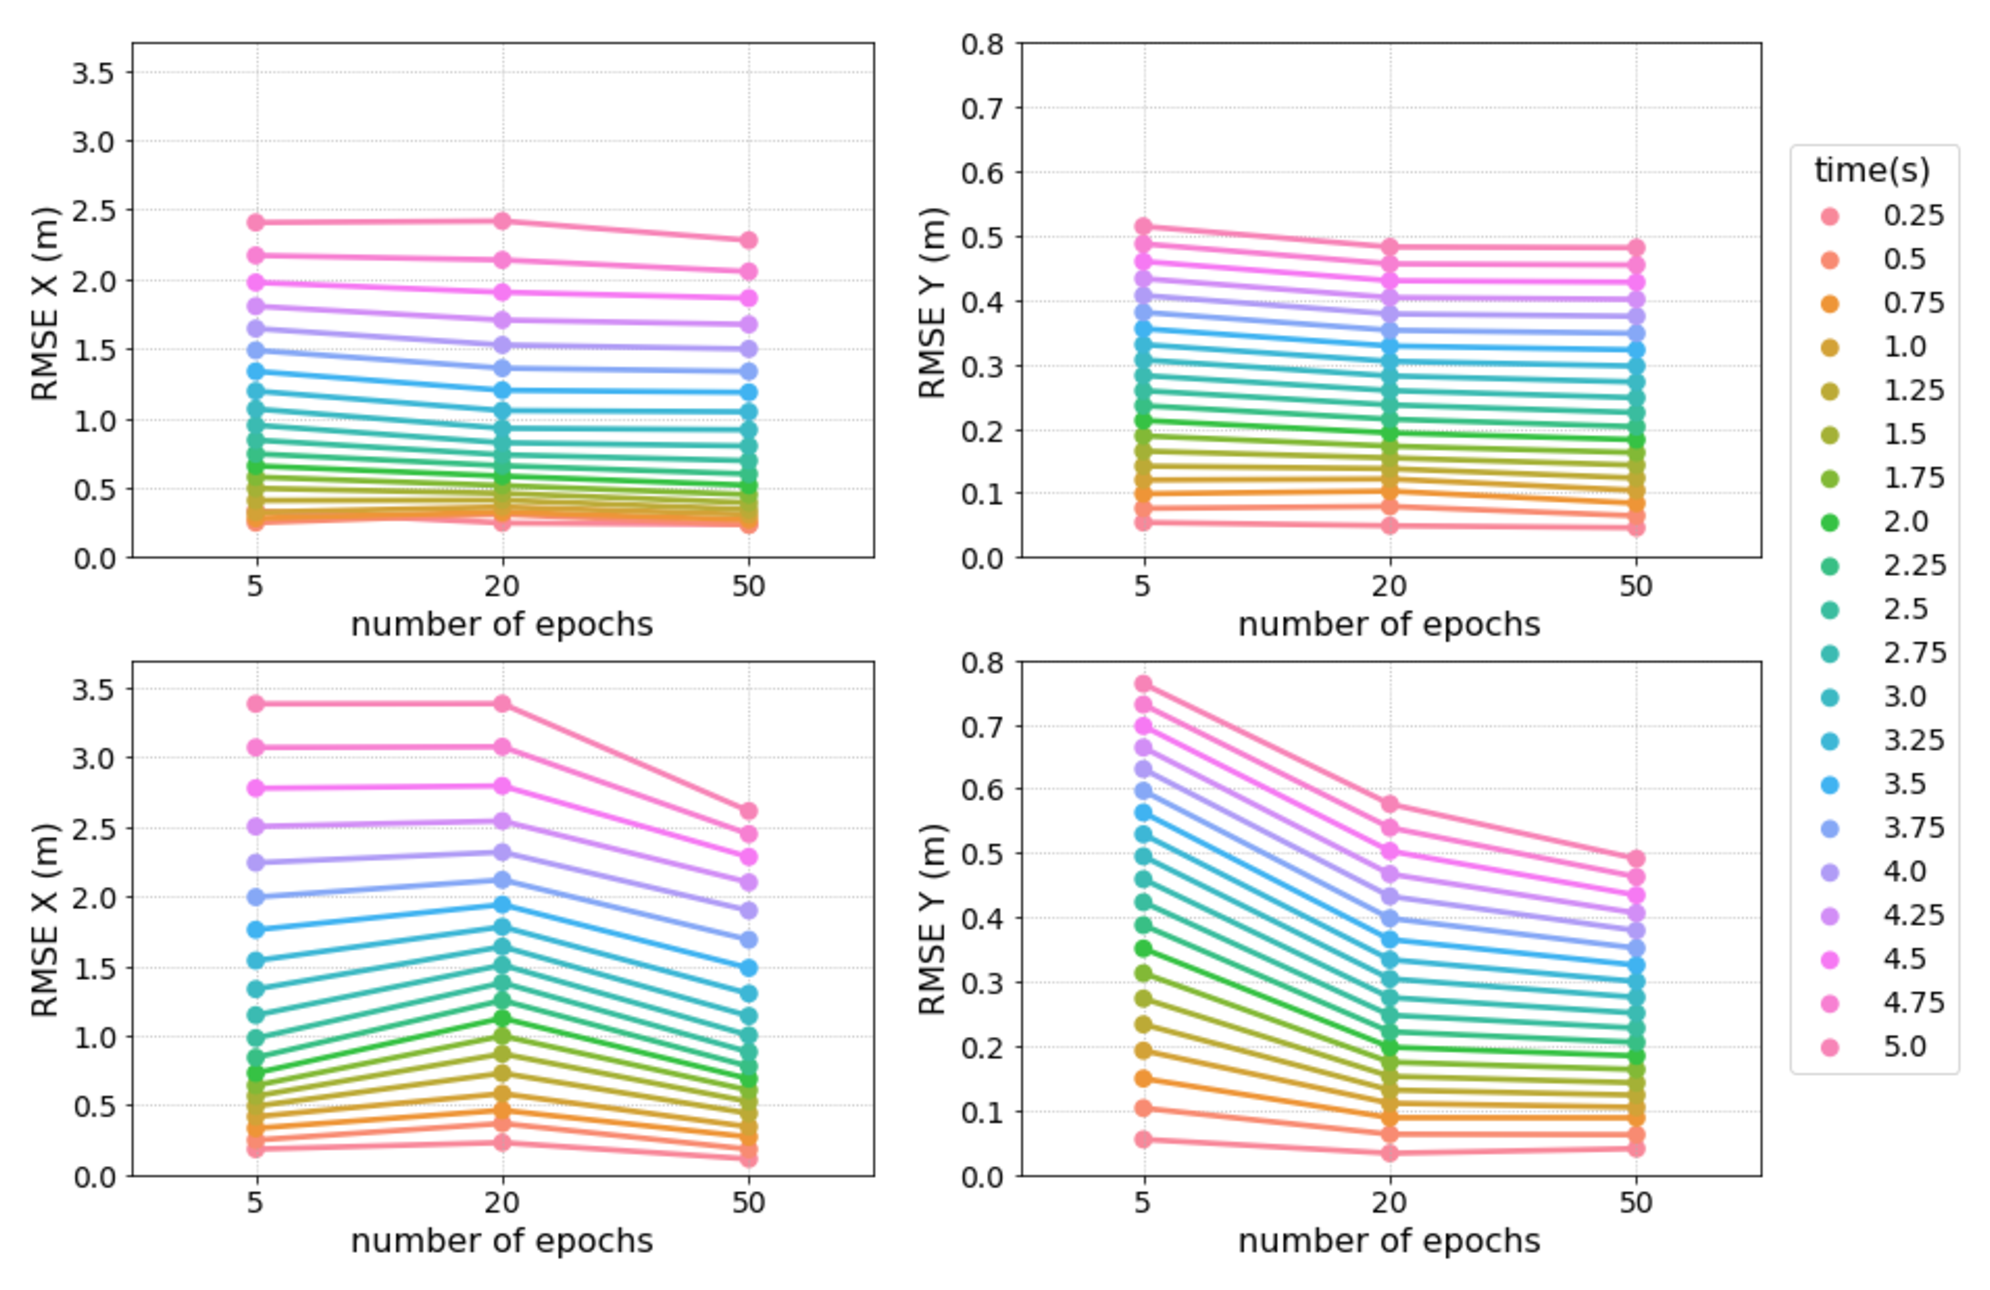
\includegraphics[width=0.95\textwidth]{imgs/lstm_layers_epochs_analysis.eps}
  \caption{Analysis of the \ac{RMSE} varying the number of layers and epochs of our \ac{LSTM} model trained on the \emph{On-board} data-set. The upper row shows }\label{fig:lstm_input_data_analysis}
\end{figure}


We varied the number of layers, the number of hidden dimensions and the number of epochs for the models to be trained.
We found, that increasing the number of layers does not improve model performance, even when training longer using more epochs.
Thus, a \ac{LSTM} model with one encoder and decoder cell each is not only the simplest network architecture but also the best in terms of accuracy as well as time needed for training.
For this architecture, we found that the network performs best with \num{150} dimensions each in the encoder and decoder cell.
Furthermore, we trained our models for \num{10} epochs as we found that training for more epochs up until \num{20} does not significantly improve the models' performance.
Fig.~\ref{fig:rmse_dev_over_epochs} visualizes this result by showing the development of the \ac{RMSE} of the \ac{LSTM} model using the \ac{SPA}-power-with-ego vector representation $(\mathbf{S}_{t}^{ego})_{t_0}^{t_N}$ as input for the training (Fig.~\ref{fig:rmse_dev_over_epochs} upper row) and validation part (Fig.~\ref{fig:rmse_dev_over_epochs} lower row) of the \emph{On-board} data-set $D_1$.
\begin{figure}[t!]
  \centering
  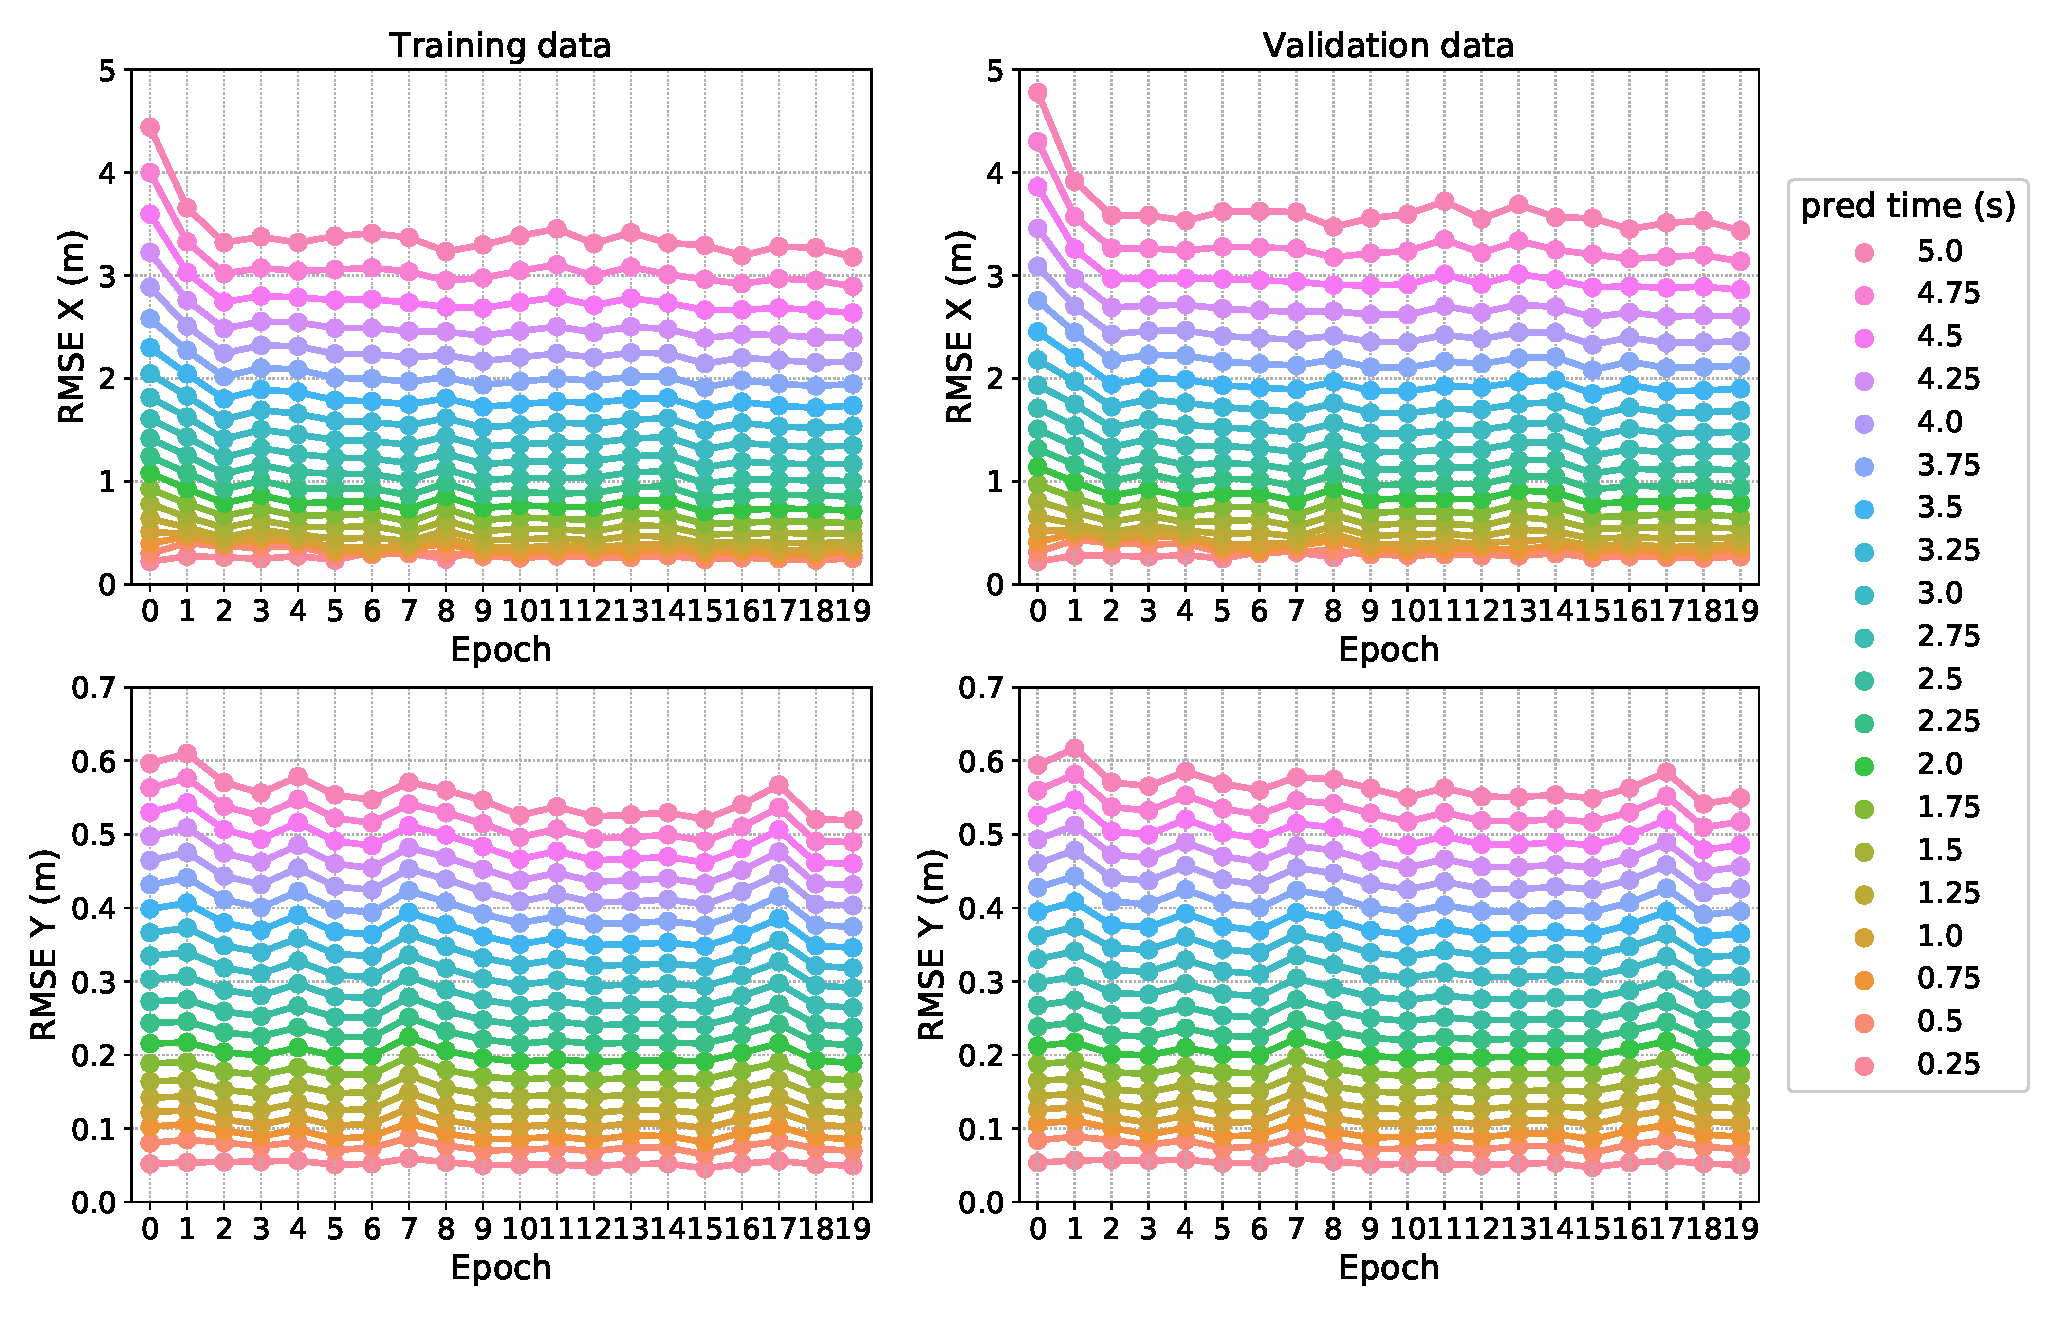
\includegraphics[width=0.95\textwidth]{imgs/rmse_dev_over_epochs.eps}
  \caption{Development of the \ac{RMSE} at every prediction time step during the training process of the \ac{LSTM} model using the \ac{SPA}-power-with-ego vector representation after each epoch on the training (upper row) and validation part (lower row) of the \emph{On-board} data-set. One observes comparable trends on both training and validation set and that the \ac{RMSE} does not significantly decrease after \num{10} epochs.}\label{fig:rmse_dev_over_epochs}
\end{figure}


\subsubsection{\ac{NEF} networks}
\label{subsubsec:hyperparam_nef}

For our \ac{NEF} networks, the main parameter influencing the models' performance are the number of neurons in the learning population (i.e. the hidden layer in terms of traditional neural networks), and the neuron model.
For simplicity, we use \acs{Nengo}'s rate-variant of the \ac{LIF} neuron model.
From the \ac{NEF}-theory \cite{Eliasmith2003} we know that increasing the number of neurons in a population yields a more accurate representation of the data encoded in the population's activity.
Thus, we expect more accurate predictions when increasing the number of neurons.
In our experiments, we found that a number of \num{3000} spiking neurons is sufficient and further increasing the number of neurons does not improve the model's prediction accuracy.
The neural weights are calculated using \acs{Nengo}'s default least-squares-optimization method with the exception, that we calculate the weights over smaller subsets of the input data for computational reasons.

\subsection{Model training}
\label{subsec:model_train}
\subsubsection{\ac{LSTM} networks}
\label{subsubsec:train_lstm}

Using the aforementioned network architecture and hyperparameter set, we train one model instantiation for each encoding scheme mentioned in Sec.~\ref{subsubsec:encoding_schemes}, whereas only the input dimensionality of the encoder cell changes when varying the representation of the input data.
Importantly, we focus on positional information as the only input for our \ac{LSTM} models in this work for reasons of consistency to make all models as comparable as possible.
Hence, we neglect for example the history of the target (or ego-) vehicle's velocity or acceleration as input here.
Between the two data-sets, the only difference between models is the auxiliary data, that is used as additional input to the \ac{LSTM} decoder cell at each time step.
For both data-sets, we use the instantaneous velocity of the target vehicle to aid the model predicting the future trajectory at every time step.
As there is no ego-vehicle present in the \emph{\ac{NGSIM}} data-set $D_2$, we use no further auxiliary data.
For the \emph{On-board} data-set $D_1$, we use the ego-vehicle's predicted acceleration and the estimated curvature of the ego-vehicle's current lane.
Although this is future information, we argue that it is solely about the ego-vehicle, which we expect to be available at the time the prediction is to happen.
We assume, that an automated vehicle, in order to safely navigate, will have an estimation of the future lane curvature as well as the acceleration values of its own planned trajectory.


\subsubsection{\ac{NEF} networks}

We train two different variants of our simpler \ac{NEF}-models using numerical input as well as the \ac{SPA}-power-with-ego and \ac{SPA}-power encoding for the \emph{On-board} and the \emph{\ac{NGSIM}} data-set respectively.
Here, we adapt the input data such that for the numerical \ac{NEF}-model, we use the vector $(x_{t_{0}}, \ldots, x_{t_{N}}, y_{t_{0}}, \ldots, y_{t_{N}}, v)$ as input with $v$ denoting the instantaneous velocity of the target vehicle.
For the \ac{SPA}-power encoding schemes, instead of flattening the whole sequence of vectors into one giant single vector, we created a single semantic vector by summing the first, middle and last element of the original vector sequences
\begin{equation}
  \hat{\mathbf{S}} =  \mathbf{S}_{t_0} \oplus \mathbf{S}_{t_{\nicefrac{N}{2}}} \oplus \mathbf{S}_{t_N} = (\hat{s}_0, \ldots, \hat{s}_{D-1}).
\end{equation}
We only sum up these vectors instead of the whole sequence $(\mathbf{S}_{t})_{t_0}^{t_N}$ to avoid the accumulation of noise in the vector representation.
Note that thereby the \ac{NEF} model using the \ac{SPA}-power representation does not use the full trajectory history but only selected time steps, namely those visualized in Fig.~\ref{fig:spa_power}.
We also include the instantaneous velocity $v$ of the target vehicle as an additional vector element, which yields $(\hat{s}_0, \ldots, \hat{s}_{D-1}, v)$ as input of our model.
To make these simpler models as comparable as possible to the \ac{LSTM} models in terms of information available to the network, we add the instantaneously velocity of the target vehicle as an additional element to the input, since there is no intermediate embedding vector here where it could be included.

\subsection{Evaluation}
\label{subsec:eval_behav_pred}
\begin{figure}[t!]
	\centering
    \subfloat[\label{subfig:lstm_rmse_all_on_board}]{%
        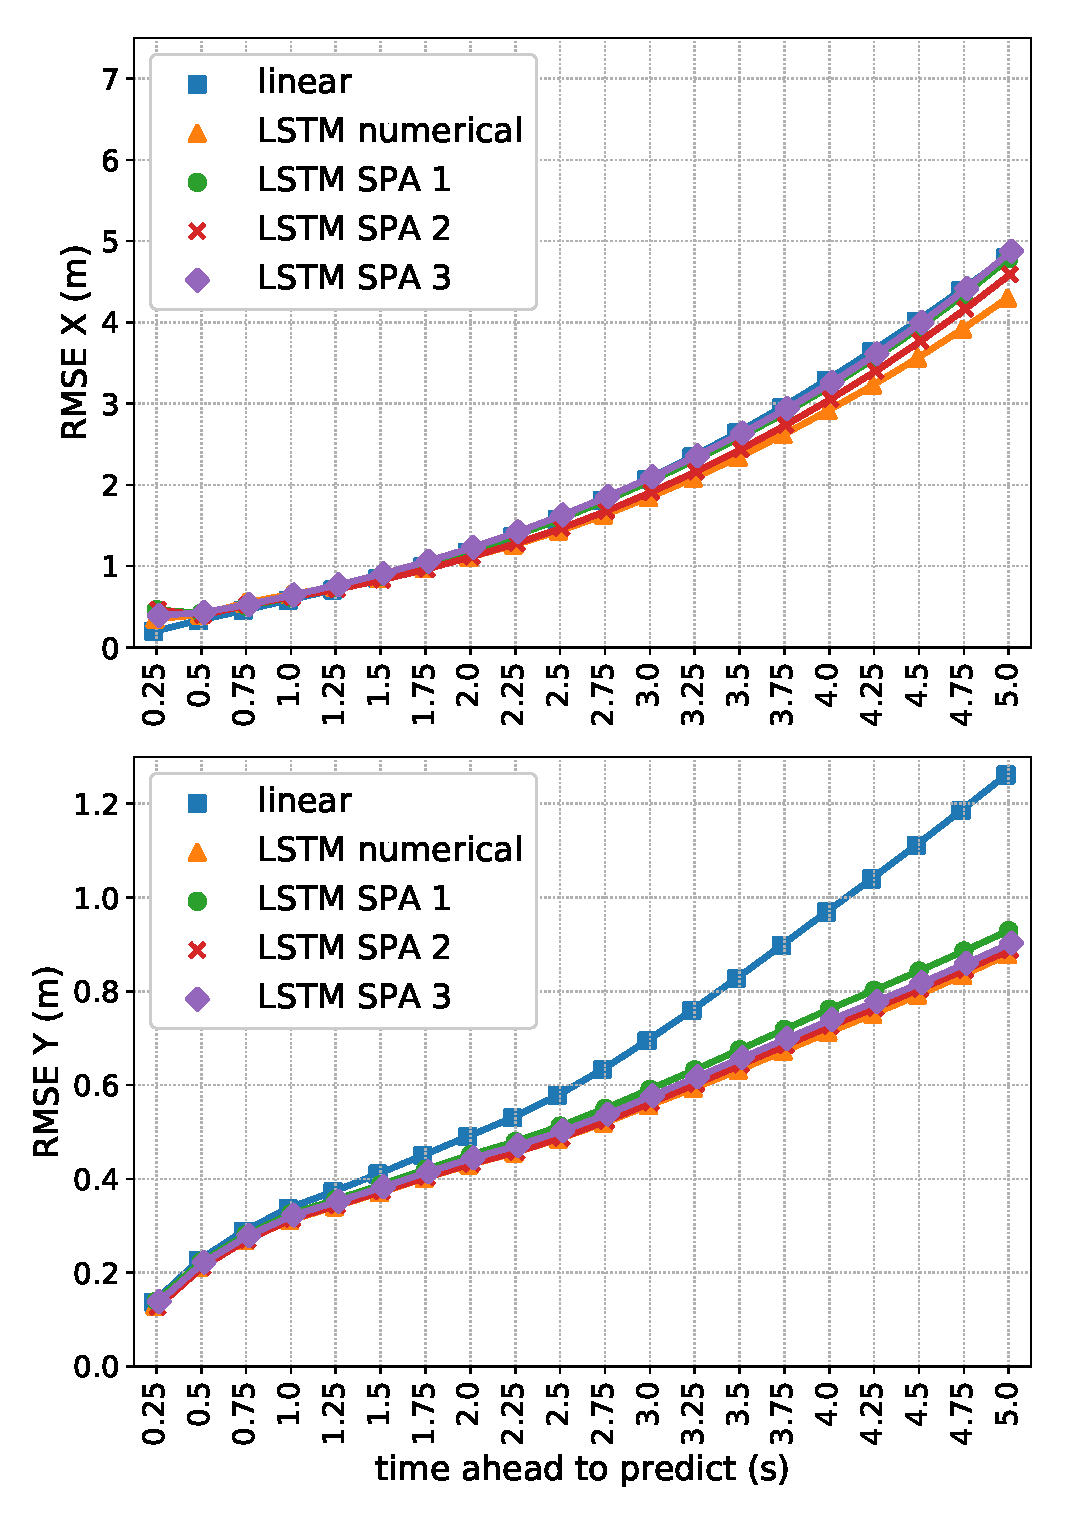
\includegraphics[width=\columnwidth]{imgs/rmse_large_all.eps}
    }
    \vspace{-0.3cm}
    \subfloat[\label{subfig:lstm_rmse_subset_on_board}]{%
        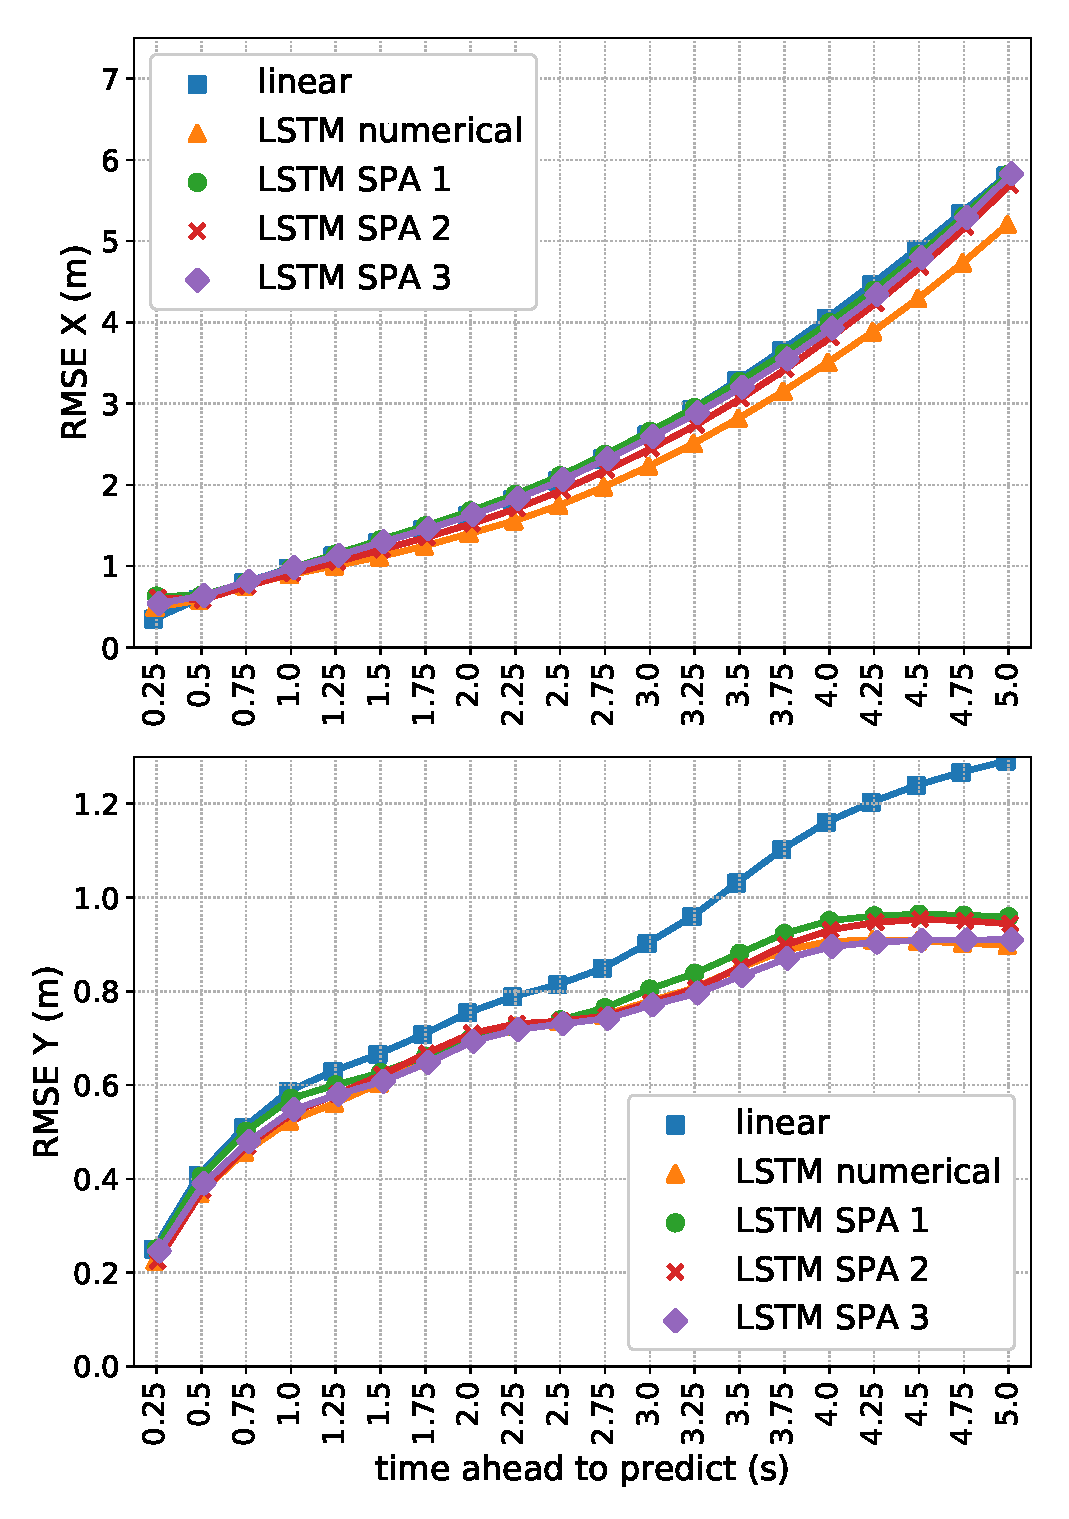
\includegraphics[width=\columnwidth]{imgs/rmse_large_subset.eps}
    }
    \caption{Visualization of the \ac{RMSE} of all \ac{LSTM} models on the \emph{On-board} data-set:~\protect\subref{subfig:lstm_rmse_all_on_board} shows the complte validation set $V_1 \subset D_1$~\protect\subref{subfig:lstm_rmse_subset_on_board} shows the subset of situations with at least \num{3} other vehicles present and distance between the target and ego vehicle lower than  \SI{20}{\meter} and between target and closest other vehicle lower than \SI{10}{\meter}.}\label{fig:rmse_on_board_all}
\end{figure}

In this section, we evaluate the performance of our models and conduct a thorough analysis of the results achieved.
For all evaluations in this section, we refer to the longitudinal and lateral direction as $x$- and $y$-direction respectively.

\subsubsection{\ac{LSTM} models}
\label{subsubsec:eval_lstm}

Fig.~\ref{fig:rmse_on_board_all} visualizes the \ac{RMSE} of all \ac{LSTM}-based models on the validation-set $V_1 \subset D_1$ of the \emph{On-board} data-set using \num{512}-dimensional vectors.
Fig.~\ref{fig:rmse_on_board_all} \textbf{(A)} shows the performance on the complete validation-set, whereas Fig.~\ref{fig:rmse_on_board_all} \textbf{(B)} depicts only situations with at least \num{3} other vehicles present, the distance between the target and the ego-vehicle being lower than \SI{20}{\meter} and the distance between the target and the closest other vehicle being less than \SI{10}{\meter}.
We observe that all approaches yield comparable results with notable differences in certain situations.
Although the \ac{SPA}-power encoding schemes tends to perform worst in $x$-direction, we observe that they perform better in $y$-direction in crowded situations with closely driving vehicles with the \ac{SPA}-power-with-ego representation ranking best along the numerical encoding scheme.

\begin{figure}[t!]
  \centering
  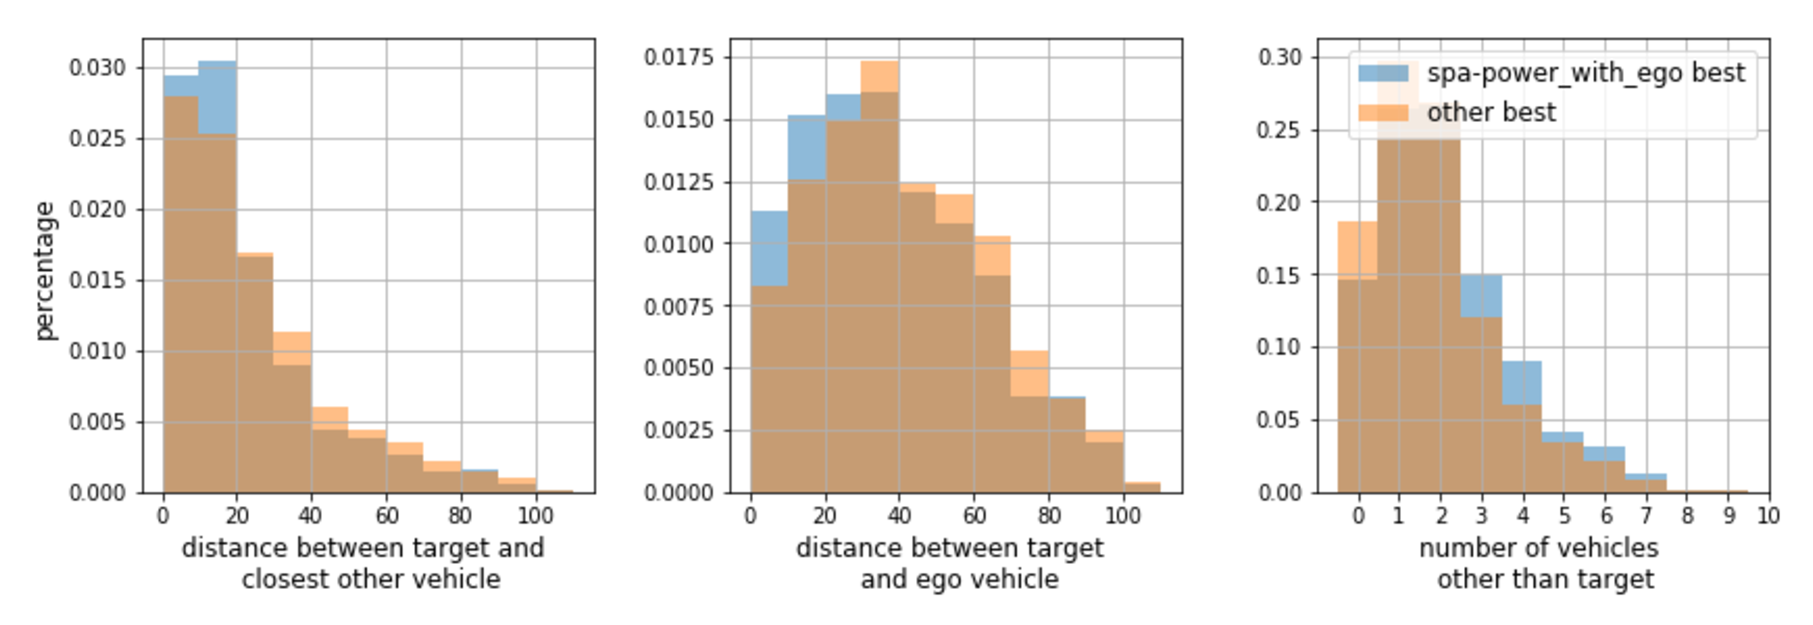
\includegraphics[width=0.95\textwidth]{imgs/histogram_on_board_revised.eps}
  \caption{Metric evaluation specifying situations where the \ac{LSTM} model using \ac{SPA}-power-with-ego representation outperforms all other approaches regarding the \acs{RMSE} in $y$-direction on the \emph{On-board} data-set $D_1$.}\label{fig:histograms_on_board}
\end{figure}

To further investigate this result, we evaluated certain metrics, chosen to characterize crowded and potentially dangerous situations, for items in the validation-set, where the \ac{SPA}-power-with-ego approach outperforms all other approaches with respect to the \ac{RMSE} in $y$-direction (see Fig.~\ref{fig:histograms_on_board}).
We observe that the ratio of situations, where the distance between the target and the ego vehicle and/or the closest other object being small is significantly higher when the \ac{SPA}-power-with-ego representation outperforms all other approaches.
Furthermore, the ratio of situations with at least \num{3} other vehicles present is also higher.
Thus, we consider these characteristics suitable candidates to serve as context variables on which our online-learning mixture-of-experts system could base its weighting decision on.
\begin{figure}[t!]
	\centering
    \subfloat[\label{subfig:lstm_rmse_512_ngsim}]{%
        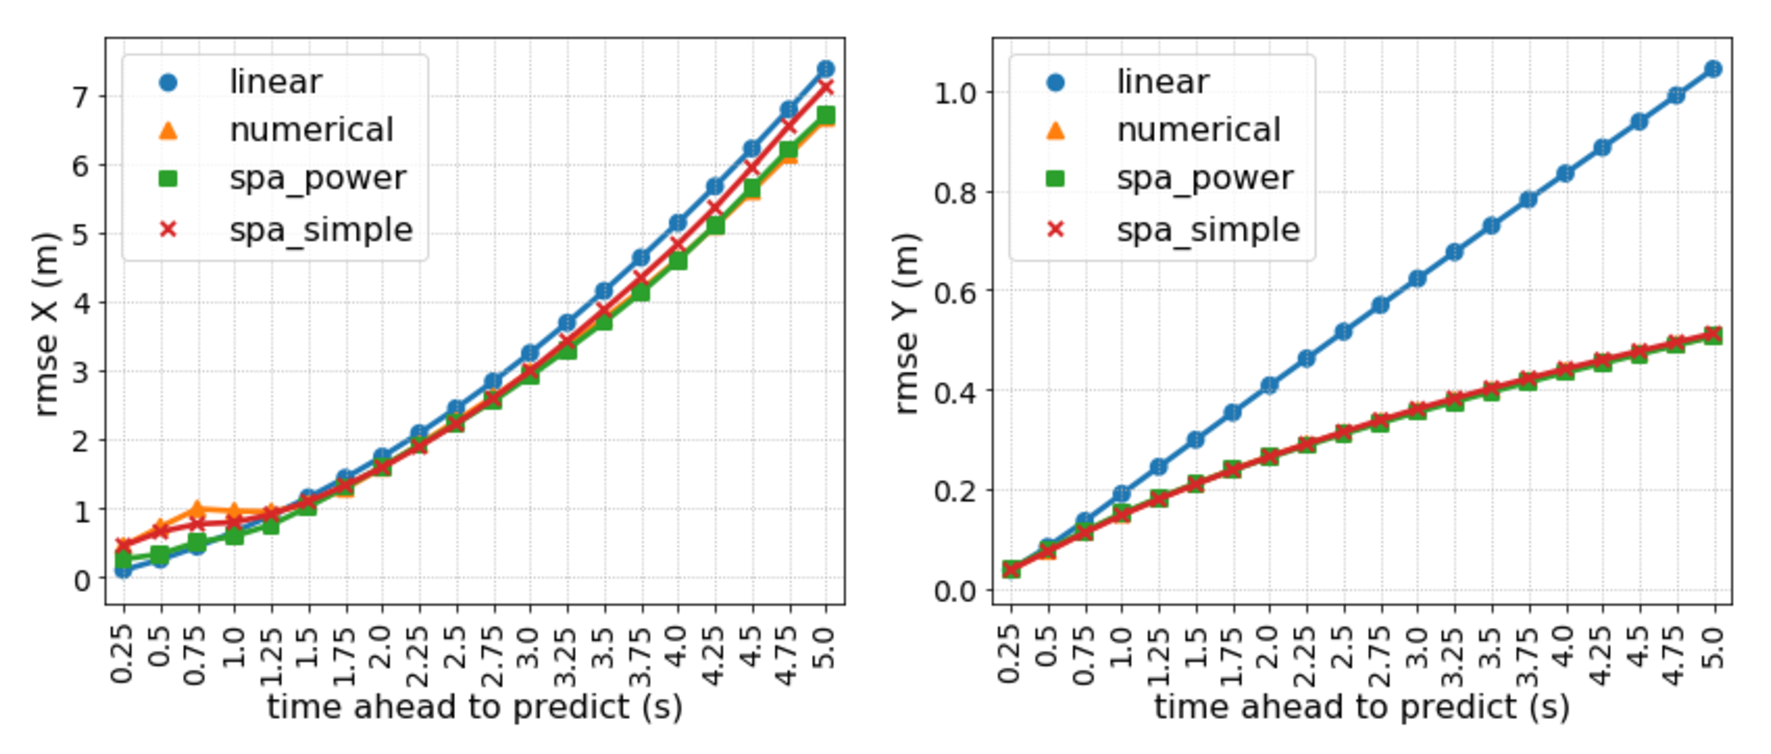
\includegraphics[width=\columnwidth]{imgs/rmse_ngsim_512_10epochs.eps}
    }
    \vspace{-0.3cm}
    \subfloat[\label{subfig:lstm_rmse_1024_ngsim}]{%
        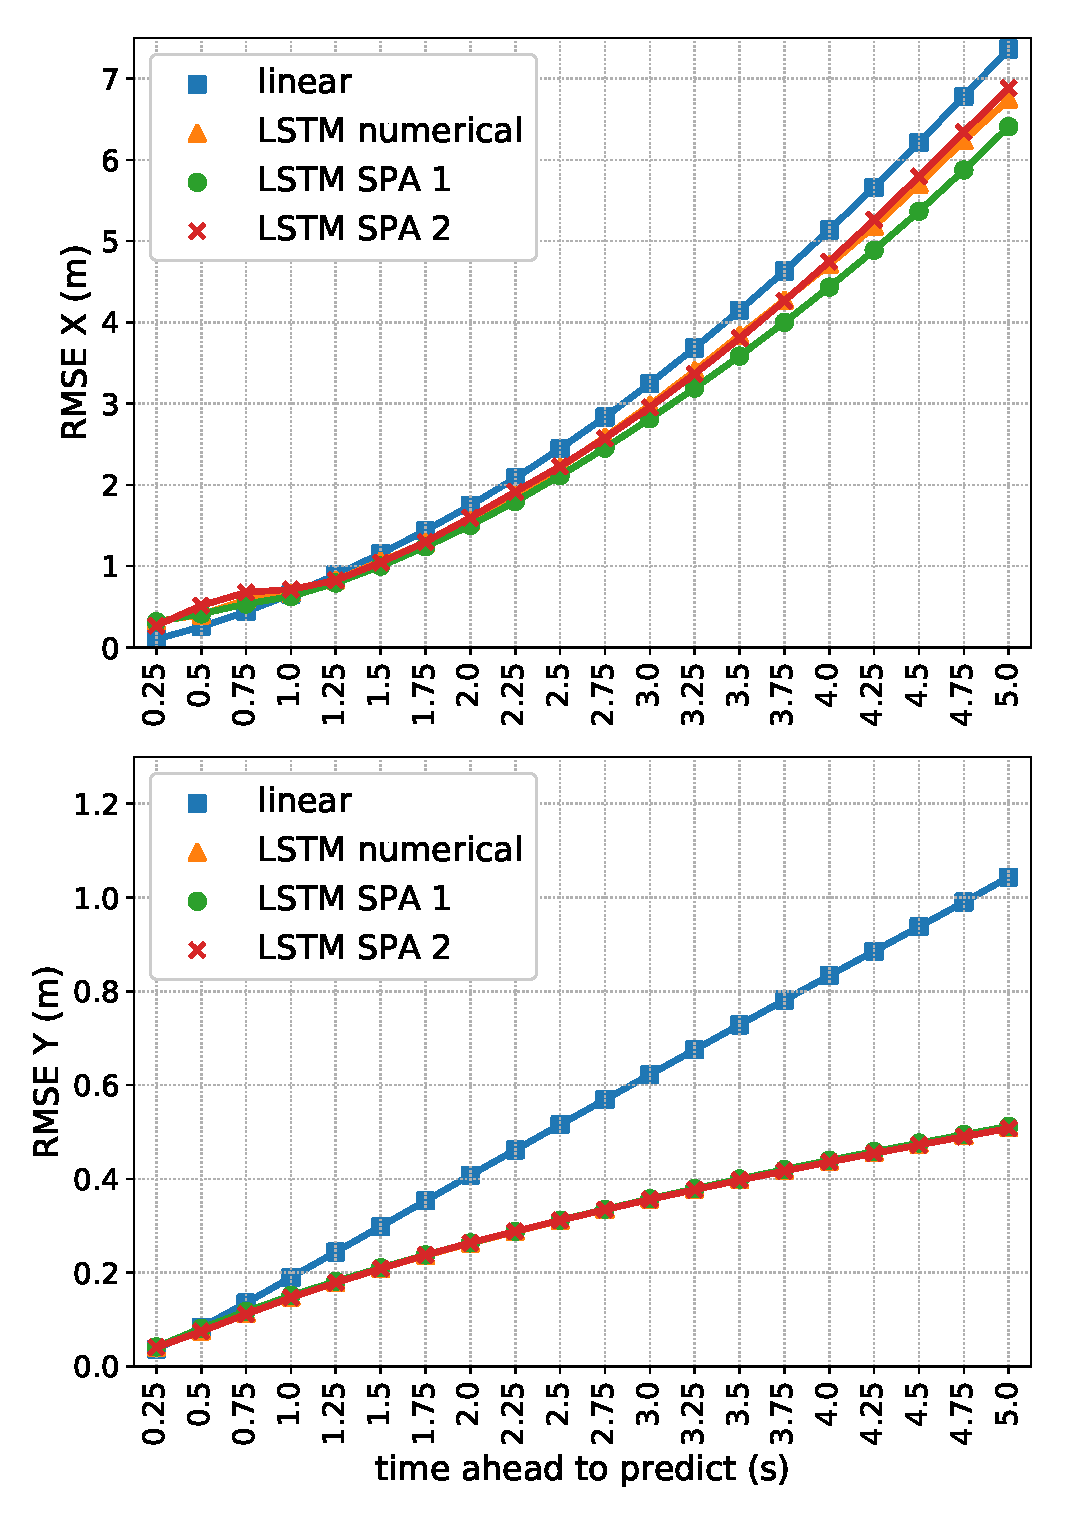
\includegraphics[width=\columnwidth]{imgs/rmse_ngsim_1024_10epochs.eps}
    }

    \caption{Visualization of the \ac{RMSE} of all \ac{LSTM} models on the \emph{\ac{NGSIM}} validation set $V_2 \subset D_2$ using~\protect\subref{subfig:lstm_rmse_512_ngsim} vectors of dimension $512$ for the \ac{SPA}-based models and~\protect\subref{subfig:lstm_rmse_1024_ngsim} using vectors of dimension $1024$ for the \ac{SPA}-based models.}\label{fig:rmse_ngsim_all}

\end{figure}

Fig.~\ref{fig:rmse_ngsim_all} visualizes the \ac{RMSE} of all \ac{LSTM}-based models on the validation-set $V_2 \subset D_2$ of the \emph{\ac{NGSIM}} data-set for \num{512}-dimensional vectors (Fig.~\ref{fig:rmse_ngsim_all} \textbf{(A)}) and for \num{1024}-dimensional vectors (Fig.~\ref{fig:rmse_ngsim_all} \textbf{(B)}).
We observe, that all \ac{LSTM} models achieve a very similar performance (almost identical in $y$-direction) with the \ac{SPA}-power representation achieving the best performance in $x$-direction being on par with the numerical encoding for \num{512}-dimensional vectors.
For \num{1024}-dimensional vectors, the \ac{LSTM} model using the \ac{SPA}-power encoding scheme even slightly outperforms all other approaches in $x$-direction, whereas we do not observe significant improvements in $y$-direction.

\subsubsection{\ac{NEF} networks}
\begin{figure}[t!]
	\centering
    \subfloat[\label{subfig:nef_rmse_512_onboard}]{%
        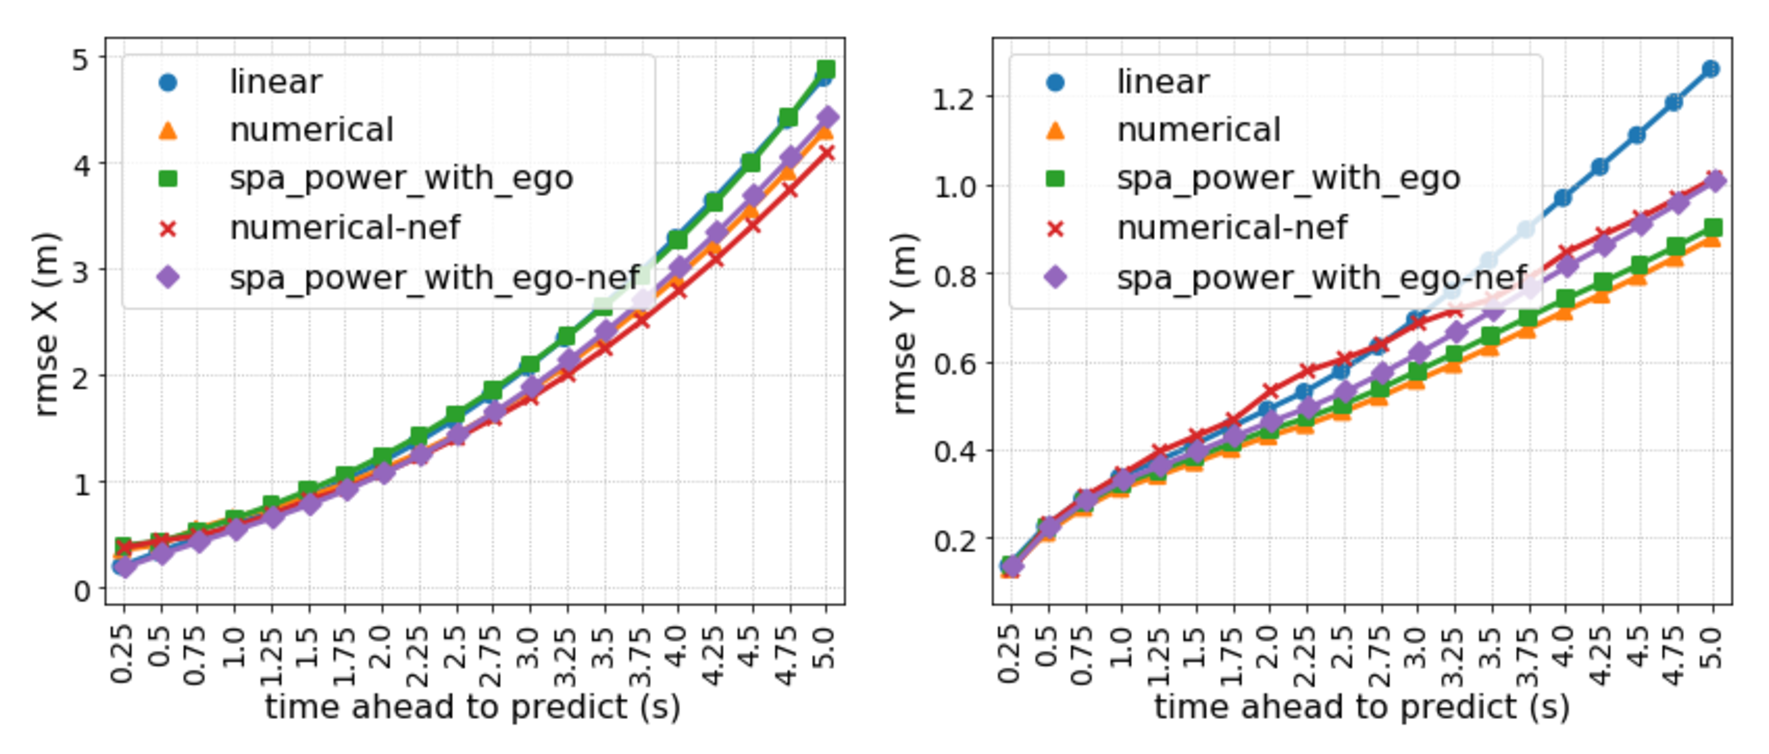
\includegraphics[width=\columnwidth]{imgs/nef_nets_on_board.eps}
    }
    \vspace{-0.3cm}
    \subfloat[\label{subfig:nef_rmse_1024_ngsim}]{%
        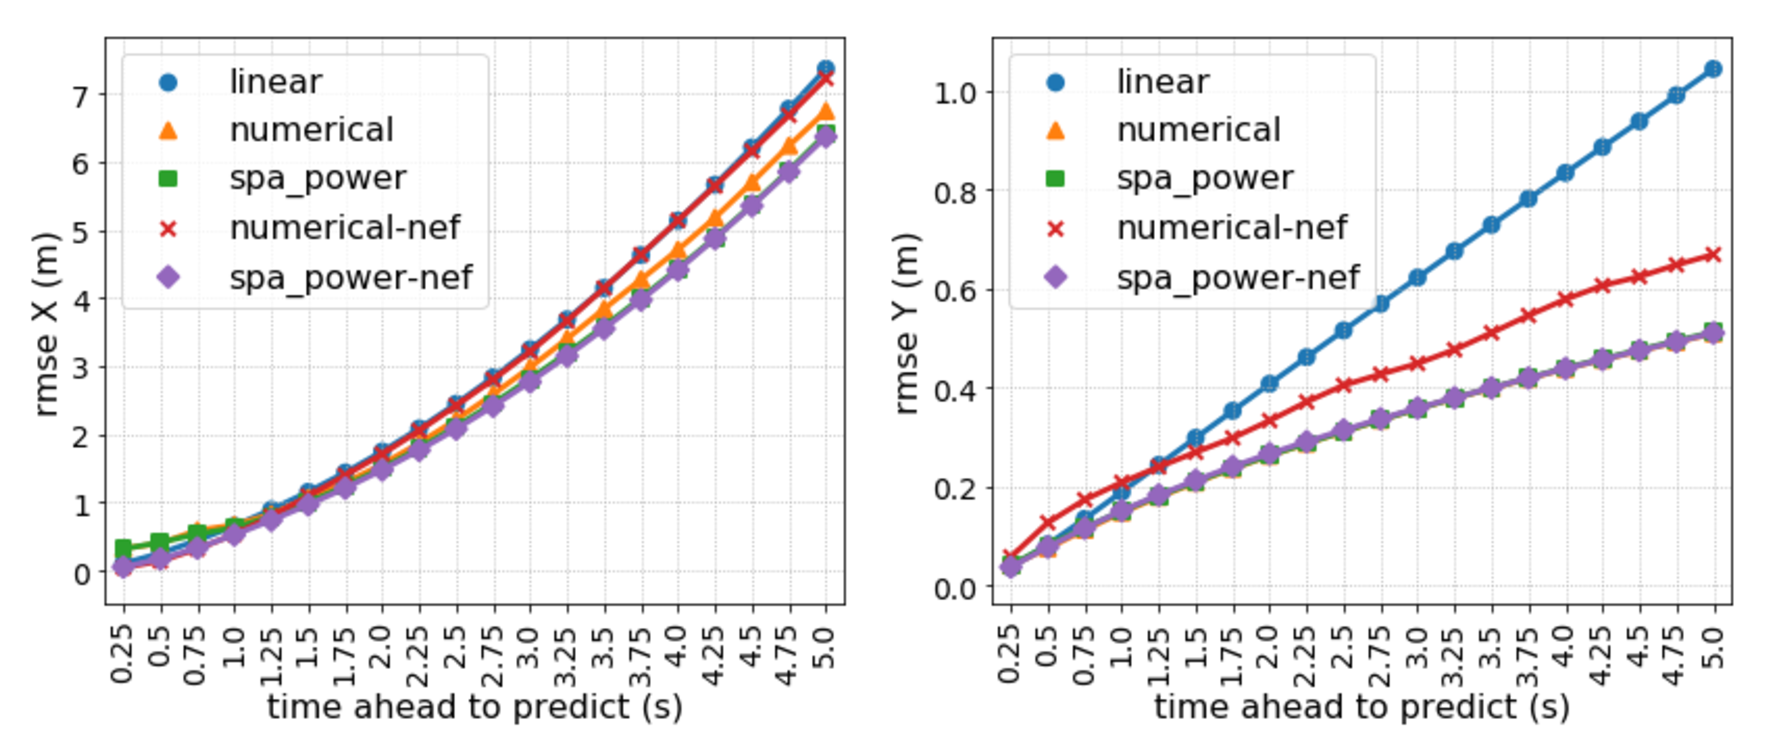
\includegraphics[width=\columnwidth]{imgs/nef_nets_ngsim.eps}
    }
    \caption{Visualization of the \ac{RMSE} of all \ac{NEF}-network models~\protect\subref{subfig:nef_rmse_512_onboard} on the \emph{On-board} validation set $V_1 \subset D_1$ using \num{512}-dimensional vectors for the \ac{SPA}-power vectors and~\protect\subref{subfig:nef_rmse_1024_ngsim} on the \emph{\ac{NGSIM}} data-set $D_2$ using \num{1024}-dimensional vectors for the \ac{SPA}-power vectors.}\label{fig:rmse_nef_nets}

\end{figure}

Fig.~\ref{fig:rmse_nef_nets} visualizes the \ac{RMSE} of our \ac{NEF}-network models on both data-sets.
The \ac{NEF}-network using the \ac{SPA}-power encoding schemes processes \num{512}-dimensional  for the \emph{On-board} and \num{1024}-dimensional vectors for the \emph{\ac{NGSIM}} data-set.
For reference, we included the performance of the most relevant \ac{LSTM} models in Fig.~\ref{fig:rmse_nef_nets} as well.
We observe that, despite a simpler network architecture and learning algorithm, the \ac{NEF}-networks achieve a performance comparable to the more sophisticated \ac{LSTM} models on both data-sets.
For the \emph{\ac{NGSIM}} data-set, the \ac{NEF}-network using the \ac{SPA}-power encoding scheme performs on par with its \ac{LSTM} model counterpart.
In this case, the \ac{NEF}-model is not only simpler, but also has access to less information as its input data is a sum of a subset of the input sequence used for the corresponding \ac{LSTM}-model.

\section{Summary}
